% Imports para generar este formato ===================
\documentclass[a4paper]{article}
\usepackage[spanish]{babel}
\usepackage[utf8x]{inputenc}
\usepackage[margin=3cm]{geometry}
\usepackage{amsmath}
\usepackage{graphicx}
\usepackage{ragged2e}
\usepackage{url}
\usepackage{multirow,tabularx}
\usepackage{hhline}
\usepackage[dvipsnames]{xcolor}
\usepackage{afterpage}
\usepackage{tocloft}
\usepackage[labelsep=period]{caption}
\usepackage{titlesec}
\usepackage{listings}

\setcounter{secnumdepth}{4}

\titleformat{\paragraph}
{\normalfont\normalsize\bfseries}{\theparagraph}{1em}{}
\titlespacing*{\paragraph}
{0pt}{3.25ex plus 1ex minus .2ex}{1.5ex plus .2ex}

% =====================================================

% Modificar diseño predeterminado del índice. =========
\addto\captionsspanish{
    \renewcommand{\contentsname}
        { \color{Blue} Índice \\         \rule{14cm}{0.1cm} \\ }
    \color{black}
}
\renewcommand{\cftsecleader}{\cftdotfill{\cftdotsep}}
\makeatletter
\renewcommand{\l@section}{\@dottedtocline{1}{1.5em}{2.6em}}
\renewcommand{\l@subsection}{\@dottedtocline{2}{4.0em}{3.6em}}
\renewcommand{\l@subsubsection}{\@dottedtocline{3}{7.4em}{4.5em}}
\newcolumntype{L}[1]{>{\raggedright\let\newline\\\arraybackslash\hspace{0pt}}m{#1}}
\makeatother
% =====================================================

% Comandos personalizados =============================
\newcommand\tab[1][0.55cm]{\hspace*{#1}}
\newcommand\gtab[1][1.5cm]{\hspace*{#1}}

\newcolumntype{Y}{>{\centering\arraybackslash}X}
\renewcommand{\arraystretch}{2}
\def\changemargin#1#2{\list{}{\rightmargin#2\leftmargin#1}\item[]}
\let\endchangemargin=\endlist 
% =====================================================

\begin{document}
\afterpage{\nopagecolor}
\pagenumbering{roman}

% Portada =============================================
\title{ 
    \centering{
        \rule{13cm}{0.05cm} \\
        
\includegraphics[scale=0.25]{tec}\\
        \textbf{Aseguramiento de la Calidad Software \\ IC-6831 } \\ 
        \rule{10cm}{0.05cm} \\ }
    \huge
    \color{Blue}\textbf{\emph{\\Segundo Avance: Futbolito}}\color{Black}
}

\author{
    \color{Blue}\Large\textbf{Profesor:  }\color{Black} \textbf{M. Sc. Saúl Calderón Ramírez}\\ [0.1cm]
	\color{Blue}\Large\textbf{Estudiantes:}\color{Black} \\
    	\textbf{Carlos M. Girón Alas} - \textbf{2014113159} \\
	    \textbf{Julián J. Méndez Oconitrillo} -  \textbf{2014121700} \\
        \textbf{Daniel A. Troyo Garro} -  \textbf{2014073396} \\
    \rule{10cm}{0.05cm}\\
    \centering{
        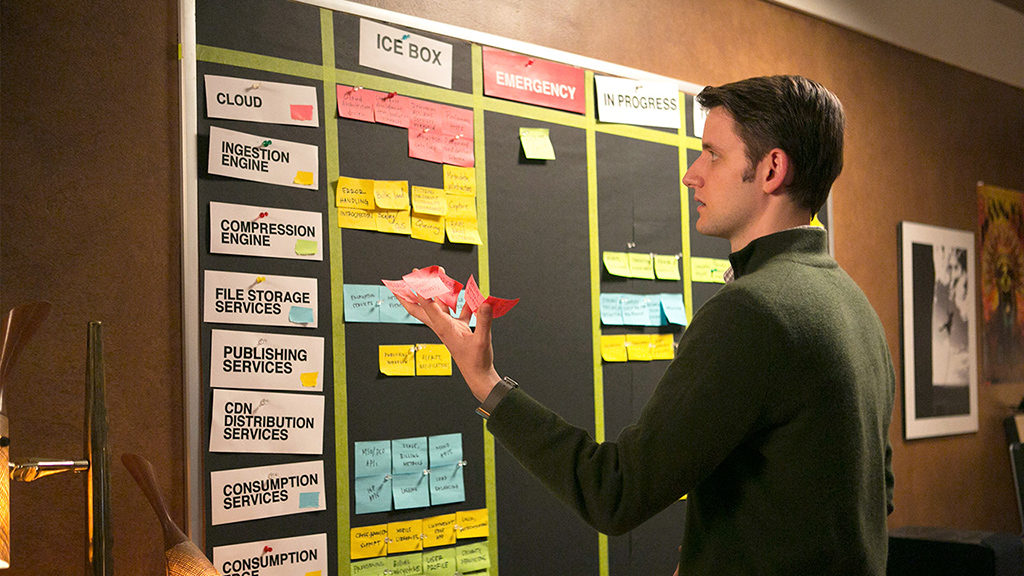
\includegraphics[scale=0.25]{scrum}}
		\date{\textbf{15 de octubre, 2016.}}
}
\maketitle
\centering{ \rule{13cm}{0.05cm} \\ 
% =====================================================

% Índice ==============================================
\newpage
\color{Blue}
\color{black}
\tableofcontents
% =====================================================

% Documento ===========================================
\justify
\newpage
\pagenumbering{arabic}

\justify 
\color{Blue}
\centering{ \rule{16cm}{0.1cm} } \\ 
\section{\textbf{Documento de Requerimientos ISO/IEC/IEEE 29148-2011}}
\color{black}

\justify

\color{Blue}
\subsection{Propósito del sistema}
\color{black}
\justify 

	\tab El Club Boca Juniors tiene la necesidad de mejorar los sistemas de análisis de los juegos con el fin de maximizar su rendimiento en la liga. Para ello, consideran que un sistema capaz de analizar los videos históricos de los partidos que ha tenido el equipo y que extraiga datos útiles de estos videos, les daría una visión más acertada de los elementos en los que pueden mejorar, tales como la solidez de su formación, el rendimiento individual de cada jugador y la forma en que interactúan los jugadores dependiendo de la posición en la que se encuentran. \\

	Todos estos datos son extraídos estadísticamente del análisis de los videos. Este sistema pretende automatizar los análisis previamente mencionados, obteniendo y mostrando de la manera más clara y asimilable posible, los datos útiles para la mejora del rendimiento del equipo. \\

\color{Blue}
\subsection{Alcance del sistema}
\color{black}

\justify

      \tab Futbolito es un sistema que busca satisfacer las necesidades del equipo técnico y administrativo del Boca Juniors en cuanto a la revisión y obtención de datos de sus juegos anteriores. \\
    
    El análisis manual de videos es una tarea exhaustiva, repetitiva y tediosa cuando es una persona el que debe hacerlo. Una situación en el que una persona tenga que ver cuatro partidos de 90 minutos de duración y analizarlos consumiría demasiado tiempo y recursos, además de no contar con la misma exactitud siempre. En cambio, dando uso a los algoritmos de análisis de visión por computadora, utilizando métodos probabilísticos y estádisticos junto con manejo de videos de forma automatizada, así como la identificación de elementos específicos en los partidos, puede reducirse la cantidad de tiempo que se invierte en el análisis de estos datos de forma sustancial. Dichos análisis puntuales se describen a continuación: \\
    
	\begin{itemize}
    	\item División de cada video en escenas: Mediante el segmentado y posterior unión de todo el video en frames unitarios, se puede detectar un corte o cambio de escena tras un análisis probabilístico del tono (\textit{hue} al pasar el frame al modelo de color HSV) de cada frame. De esta manera, se puede separar un video de un partido en distintos videos donde cada una es una escena del video original, esto para una selección más precisa de momentos específicos de un partido. 
        \item Obtención de la duración de cada escena: Necesidad ligada a la anterior respecto a la selección de escenas. La determinación de este valor se da al calcular el número de frames por segundo y obtener la variable del tiempo.
        \item Eliminación de escenas irrelevantes como tomas del público, anuncios publicitarios, entre otros. El propósito principal de esto es el de filtrar segmentos del video que no aporten valor agregado al análisis tales como tomas del público, las cuales no aportan datos útiles que permitan generar un informe de la consistencia de la formación del equipo  o de demás factores requeridos.
       	\item Análisis de la consistencia y solidez de la formación del equipo en la cancha, pasando de la línea defensiva, medio campo y línea ofensiva. Mediante técnicas de \textit{computer vision}, se logrará la identificación de cada jugador en una toma y el análisis colectivo de cada toma, se podrá saber la posición del jugador en el campo de juego a lo largo de todo el partido y realizar un análisis estadístico de la influencia que tiene en el resultado final del partido este tipo de variables. 
        \item Análisis del rendimiento individual de cada jugador: Tal y como se especificó en el punto anterior, tras realizar análisis estadísticos y probabilísticos sobre los datos obtenidos del análisis de posición de cada jugador, se puede derivar el desempeño que tuvo el jugador durante el partido y maneras de poder optimizarlo. 
        \item Análisis del posicionamiento de cada jugador y su relación con la formación general del resto del equipo: Mediante identificación de la posición de cada jugador en el campo de juego en el video se puede obtener un conjunto de datos que representen el movimiento del jugador a lo largo del campo de juego durante todo el video y así poder determinar variables determinantes para aproximar un rendimiento del jugador, tales como velocidad, número de veces que rompió la formación general, número de \textit{Fuera de juego}, entre otras.  
        \item Generación de informes con los datos obtenidos durante todo el funcionamiento del sistema: Los usuarios principales del sistema, los cuales son el cuerpo técnico y junta administrativa del club Boca Juniors. Esto requiere que los datos obtenidos sean presentados de una manera clara, directa y explícita, brindando al usuario la mayor capacidad de comprensión de los reportes obtenidos. Por esto, el sistema generará archivos conteniendo los informes en formato .csv, .xlsx, .docx o pdf, donde se muestre el rendimiento general del equipo, así como los resultados de la segmentación temporal del video. 
    \end{itemize}
    
	\tab La aplicación principal de este sistema es la del análisis automatizado de videos de partidos de fútbol, principalmente hecho para el club Boca Juniors. Los objetivos y necesidades específicas del cliente ya han sido definidas en la sección anterior como ítems. Mediante dichos requerimientos se espera satisfacer las necesidades del cliente respecto a la obtención de datos estadísticos del equipo Boca Juniors. \\

\color{Blue}
\subsection{Panorama general del sistema.}
\color{black}
\justify 

\color{Blue}
\subsubsection{Contexto del sistema}
\color{black}
\justify 

	\tab La aplicación tiene varias etapas. Como es importante y pertinente que el sistema sea fácilmente accesible para el usuario que lo requiera en cualquier momento, se seleccionó la interfaz en un ambiente web, de manera que se pueda accesar desde cualquier equipo con un explorador web. En cuanto al desarrollo de las partes internas o back-end del sistema, es un servidor en java que atiende consultas de los clientes web y las atiende pertinentemente. \\
    
    Las funcionalidades generales que tiene la aplicación web son la carga de un video y la selección de un tipo de análisis sobre el video subido al servidor. Una vez analizados los datos debe mostrársele al usuario los resultados del análisis en una forma amigable que sea fácil de entender. En el caso de la segmentación temporal, debe notarse cuáles son los momentos que presentan uno de los cambios de escena y cuáles no. En cuanto a los elementos de la identificación de jugadores se deben presentar los datos estadísticos de rendimiento de los jugadores y de posiciones adecuadas de acuerdo a la formación y a su desplazamiento por la cancha. Demás variables que el cliente considere apropiadas serán definidas en iteraciones posteriores del proyecto. 


\color{Blue}
\subsubsection{Funciones del sistema}
\color{black}
\justify 

	\tab El sistema principal debe constar de 3 elementos básicos. El primero es una aplicación web previamente descrita en la que el usuario puede acceder a las funcionalidades del sistema. Este primer elemento debe permitirle al usuario visualizar el video subido, así como los videos devueltos por el servidor; cargar videos para segmentación temporal y enviado al servidor, cargado de archivo \textit{ground truth}, el cual puede ser de distintos formatos definidos más adelante, poder seleccionar los puntos de corte de manera manual mediante una interfaz cómodo y dinámica y poder descargar los informes generados así como los videos productos de la segmentación. \\ 
    
    El segundo elemento es el servidor web que debe tener una disponibilidad activa alta de forma que en casi cualquier momento se pueda usar las funcionalidades del sistema. Este elemento funciona como punto intermedio entre la plataforma web y la biblioteca de análisis de videos, enviando los videos e informes de un punto a otro y sirviendo como plataforma de ejecución del programa principal JAVA que realiza la lectura, análisis y segmentación del video. \\ 
    
    El tercer y último elemento de mayor relevancia es la biblioteca utilizada para los análisis que se hacen sobre los videos. Dicha biblioteca funciona en conjunto con las biblioteca preestablecidas de OpenCV, framework multiplataforma que permite implementar algoritmos de \textit{computer vision} y análisis de videos de manera simple y eficaz,  para que ocurran los análisis probabilísticos y estadísticos de histogramas para los frames del video que desprenden otros datos de suma importancia que se pueden muestrear y aplicar distintos métodos  que encuentren relaciones entre elementos. De momento la aplicación se limitará al análisis de videos de juegos de fútbol y la generación de datos estadísticos de los mismos, de forma que el uso que se le da a estos datos está limitado a lo que los usuarios decidan hacer con ellos. Esto implica que la subida de videos en los que no se presente un juego de fútbol no extraerá datos significativos al no poder identificar a los jugadores en el campo de juego y no obtendrá un análisis estadístico, mostrándosele un mensaje de advertencia. \\


\color{Blue}
\subsubsection{Características del usuario}
\color{black}
\justify 

	\tab Los usuarios hacia los que está dirigida esta aplicación son el equipo técnico y administrativo  del Boca Juniors. Sin embargo, la funcionalidad del sistema de análisis de videos podría tener aplicaciones para otros usuarios que den uso a la interpretación de señales. Este tipo de usuario final es muy amplio ya que es todo aquel que comprenda la aplicación que tiene los algoritmos de \textit{computer vision} en el procesamiento de videos de partidos de fútbol y que tenga acceso a una terminal con un navegador web, por lo que un futuro el sector meta podría aumentar a otros clubes de fútbol o a libre acceso. En cuanto al equipo de operación, los elementos internos del servidor son manejados por una pareja de administradores o moderadores que se encargarán de casos anormales que el sistema mismo no es capaz de manejar. Por otra parte, en cuanto al mantenimiento de la aplicación, el equipo de mantenimiento consiste en dos técnicos que se encargan de la recolección de datos relevantes respecto al uso del sistema, y que están a cargo de posibles proyectos de integración, así como el modelado de nuevas funcionalidades y la integración de esta aplicación con otras que tengan elementos análogos que pueden aprovecharse. \\

\color{Blue}
\subsection{Requerimientos funcionales}
\color{black}
\justify 

	\tab Los requerimientos funcionales se definen a continuación. 
    
   	\subsubsection{Acceso a la aplicación (Prioridad Media)}
    	En primer instancia el sistema debe tener una interfaz de usuario disponible en línea y esta debe contar como \textbf{mínimo} con la opción de subir el video y una vez que un video es seleccionado, la posibilidad de reemplazarlo o de enviarlo a análisis. Se le debe restringir al usuario la selección de archivos multimedia únicamente, siendo los siguientes formatos los inicialmente permitidos: .mp4, .avi, y . wav.
        
    \subsubsection{Subida del video (Prioridad Alta)}
    	Compuesta de las siguientes etapas: \\
		
        \paragraph{Opción de subir o reemplazar: (Prioridad Media)}
     	La interfaz debe tener un botón claramente identificable que le permita subir un video al servidor sin la necesidad de hacer ningún estilo de comprobación manual por parte del usuario. . \\ 
        
        \paragraph{Tiempo de espera: (Prioridad Baja) }
        Durante el tiempo de subida del video al servidor, cuya duración es directamente proporcional al tamaño del video en cuestión, debe mostrársele al usuario una barra de avance que le informe cuánto tiempo estimado falta para que concluya la subida y cuánto tiempo ha transcurrido. \\
        
       	\paragraph{Subida del video: (Prioridad Alta) }
        El sistema debe contar con el sistema de verificación que evita que el usuario suba un archivo que no sea multimedia con formato de video. En las características actuales, el sistema tiene soporte a .mp4, .wav y .avi, con búsquedas a añadir otros formatos. \\
        
        \paragraph{Visualización del video: (Prioridad Media) }
        Tras subir el video a la aplicación web, esta debe mostrar un reproductor de video en el que el usuario pueda visualizar el video. Asegurándose de que la integridad del video no se vio comprometida en la subida del mismo y que cumpla con las características deseadas para el ingreso del mismo al componente del servidor que analizará el video. \\

		\paragraph{Errores: (Prioridad Baja) }
		El sistema debe mostrar al usuario un mensaje informativo sobre la naturaleza del error presentado, de una forma agradable. En el caso por ejemplo de un video subido con un formato no soportado, muestra el error. En caso de un problema en la subida del video, debe reportarse igualmente que el sistema encontró una dificultad en la subida que puede tener diversas naturalezas, en caso de que el sistema no esté disponible debe presentarse dicha información claramente y negar el uso del sitio durante el periodo de mantenimiento.  \\

	\subsubsection{Envío del video a análisis (Prioridad Media) }
    	Compuesta de las siguientes etapas: \\
        
    	\paragraph{Opción analizar: (Prioridad Media) }
        	La interfaz tiene un botón que permite al usuario enviar el video subido a análisis. Este botón debe ser habilitado cuando hay un video actual subido para ser analizado o al menos debe presentar un error cuando un archivo no ha sido subido. \\
            
        \paragraph{Selección de punto de corte manual: (Prioridad Baja) } 
        	Una vez cargado el video, se le debe permitir al usuario seleccionar unO o varios puntos entre los frames mostrados en pantalla (los cuales son obtenidos tras dividir el video por el programa java del servidor) y así el análisis entre videos se omitiría, ya que las escenas serían extraídas en base a lo seleccionado por el usuario. La selección de al menos un punto de división entre escenas anulará la segmentación temporal automática y el video se dividirá únicamente en las escenas determinadas por el usuario. \\
            
        \paragraph{Tiempo de espera: (Prioridad Baja)}
        	Una vez presionado el botón de enviar a análisis, el sistema debe presentar de nuevo un estimado del tiempo que tomará el análisis del video para que el usuario tenga una idea del tiempo transcurrido y del posible tiempo restante. \\
            
		\paragraph{Errores: (Prioridad Baja) }
        	En caso de que el análisis del video presentara algún error, debe presentarse un mensaje de error informativo al usuario. En caso de que el proceso se cierre o se actualice la página, debe redirigirse a la página de inicio por defecto, donde el usuario puede volver a comenzar el proceso de análisis sin la necesidad de volver a subir el video, o puede elegir reemplazar el video actual con un nuevo video en el botón de Subir video descrito en el requerimiento funcional 3.4.2.  \\
     
        \subsubsection{Servidor web (Prioridad Media) }
     	
        El servicio web en java debe estar disponible en el momento que la página es utilizada. Esto implica que en caso de un error en el servidor, este debe informarse en la página web. El servicio cuenta con sistemas de respuesta únicamente a requests identificados de la página, por lo que la conexión se asegura como segura. \\ 
            
        \subsubsection{Algoritmos de segmentación temporal (Prioridad Alta)}
      	
        Los resultados que presenta el sistema una vez analizado el video provienen de un análisis de histogramas  obtenidos de cada cuadro o \textit{frame}en los que es divido el video que se subió para ser analizado. Todos estos algoritmos son implementados por el programa de java ejecutándose en el servidor con la ayuda de funciones propias de la biblioteca \textit{OpenCV}. De esta forma, se presentan a continuación dichas funciones. \\
        
      \paragraph{Algoritmo de Bhattacharyya (Prioridad Alta)}
      
      El algoritmo de Bhattacharyya consiste en la obtención de la medida de distancia entre dos histogramas mediante el cálculo de un coeficiente homónimo y una posterior normalización utilizando un coeficiente obtenido con valores de los histogramas, tales como la media. La implementación de este algoritmo se realizará para calcular el grado de \textit{diferencia} entre dos imágenes y así determinar si ocurre un \textit{corte} o cambio de escena entre ellas, así poder separar el video en dos escenas en tal punto. \\
      
      Mediante este algoritmo se calcula un arreglo de disimilitud entre cuadros del video consecutivos, almacenando así los valores obtenidos mediante el algoritmo de la distancia de Bhattacharyya.  \\     
      
        \paragraph{Teorema de los tres sigmas (Prioridad Alta)}
      	
        El teorema de los tres sigmas tiene una aplicación directa en el proceso de segmentación temporal y la obtención de los puntos de corte o de división de escenas. Este teorema es necesario para obtener en qué puntos del video ocurre un cambio de escena y así permite que mediante algoritmos de bibliotecas multimedia nativas del API de JAVA se logren la generación de nuevos videos, escenas que serán enviadas al usuario  a la aplicación web. 
        
     
     \subsubsection{Obtención de resultados (Prioridad Media)}
     
        	Una vez completado el proceso de análisis, el sistema cambiará su configuración para presentar los resultados obtenidos. Ahora, en lugar de presentarse los elementos iniciales, se presentarán un botón de avance y un botón de retroceso que permiten al usuario avanzar entre los frames procesados, y se muestra una etiqueta que le indica al usuario si en ese frame se presentó un corte. Se considera un corte a aquel frame justo después de uno con una escena completamente diferente. Compuesta de las siguientes etapas: \\ 
            
    	\paragraph{Obtención de escenas ordenadas por posición: (Prioridad Media)}
        	La interfaz de la aplicación web debe mostrarle al usuario los N videos obtenidos de la segmentación del video con una etiqueta que indique su posición en el video inicial y la capacidad de poder visualizarlos en la aplicación, así como descargar un archivo comprimido que contenga todos estos videos. El archivo podrá ser de formato .zip. \\
            
        \paragraph{Visualización de cortes detectados (Prioridad Media)} 
        	En algún punto de la aplicación web se le debe mostrar al usuario el número de cortes realizados al video original. Este es un valor simple, el cual está compuesto de un simple valor entero positivo. \\
            
        \paragraph{Visualización de escenas (Prioridad Media)}
        	Al igual como sucede con el video subido, la aplicación web tiene que permitirle al usuario visualizar cada una de los videos de las escenas devueltas tras la segmentación.  \\
            
        \paragraph{Muestreo de información obtenida del análisis: (Prioridad Baja)}
        	El sistema debe de mostrar la información en la página web obtenida del análisis del video. Estos valores pueden mostrarse de manera tabulada o mediante algún formato adecuado.    \\ 
            
        \paragraph{Descarga del informe en distintos formatos: (Prioridad Baja)}
        	El sistema debe de permitir la descarga del informe en formatos variados tales como .xlsx, .docx, .pdf o .csv.   \\ 
            
    \subsubsection{Subida del archivo de ground truth (Prioridad Alta)}
    	Compuesta de las siguientes etapas: \\
		
        \paragraph{Opción de subir o reemplazar: (Prioridad Alta)}
     	La interfaz debe tener un botón claramente identificable que le permita subir un archivo de ground truth al servidor sin la necesidad de hacer ningún estilo de comprobación manual por parte del usuario. \\ 
        
        \paragraph{Opcionalidad del Ground Truth (Prioridad Media)}
        La subida del archivo de ground truth es opcional, junto con el envío del video (que no es opcional). Al enviar un archivo a esa dirección, comienza un análisis con el servidor que devolverá si el análisis del video es satisfactorio respecto a lo especificado por los archivos de \\ 
         
        \paragraph{Extensiones del Ground Truth (Prioridad Baja)}
		 Los archivos válidos para el archivo de ground truth son únicamente .xml, .json, .csv, .yaml, .txt\\ 
         
    \subsubsection{Análisis de ground truth (Prioridad Alta)}
    	Compuesta de las siguientes etapas: \\
		
        \paragraph{Presentación del análisis comparativo: (Prioridad Alta)}
     	Presentará la comparación entre los resultados obtenidos y los datos introducidos por el ground truth para generar una cuantificación de falsos positivos y negativos. \\ 

        \paragraph{Formato del archivo: (Prioridad Baja)}
     	La forma en la que esté diseñado manualmente el archivo de ground truth debe seguir el formato json para mostrar el frame en el que ocurrió el cambio, el número de frame y la cantidad de frames que hubo entre cortes. El formato mínimo que debe aceptarse es .csv parseado de la siguiente forma: \\
        
\centering { frame inicial, fram final, tipoCorte, tipoEscena } \\

\justify

\tab 		Las columnas frame inicial y frame final deben ser valores enteros positivos, puesto que indicarán el número de frame en el que inicia y termina una escena. Las columnas adicionales no se tomarán en cuenta para el muestreo de resultados. \\


\justify

\color{Blue}
\subsection{Requerimientos de usabilidad}
\color{black}  %%AÑADIR MÉTRICAS
\justify 
	Los requerimientos de usabilidad respecto a la experiencia del usuario se describen a continuación. 

       \subsubsection{Entendibilidad}
    	El usuario debe comprender fácilmente lo que ocurre después de cada acción que realiza en el sistema así como el flujo general de las acciones del mismo. Se asegurará mediante una métrica de \textbf{completitud de la descripción} que el usuario logre dar un puntaje positivo a la facilidad de la comprensión del funcionamiento general del sistema. Esta encuesta será realizada mediante la herramienta Google Forms y sus valores serán obtenidos en la versión beta de la plataforma. Algunos componentes que influenciarán la entendbilidad del sistema son:  
        
          \paragraph{Mensajes de éxito, advertencias y errores} 
          
\tab El sistema debe de mostrar de manera apropiada y entendible mensajes apropiados al comportamiento y reacción del sistema ante una entrada por parte del usuario. Los mensajes que debe de mostrar de la manera más clara posible son:
          

          \paragraph*{\gtab 1.5.1.1.1 Error} Si se presenta un error, debe mostrársele un mensaje con los detalles y las opciones que tiene a continuación.
      
          \paragraph*{\gtab 1.5.1.1.2 Advertencia} Si la acción que está por realizar tiene consecuencias no tan evidentes, un mensaje de advertencia deberá aclarar los que esto implica sin volverse un distractor ni obstruir el funcionamiento del sistema. 
          
          \paragraph*{\gtab 1.5.1.1.3 Éxito}  Si un proceso ha concluido con éxito, el usuario debe ver los elementos que se completaron y las opciones siguientes para continuar en el uso de la página si así lo desea.  
       
        \subsubsection{Operabilidad}
    	El sistema debe de permitir al usuario interactuar con él de una manera eficaz y que ningún dato de entrada inesperado colapse el funcionamiento. Por esto, se utilizará la métrica de \textbf{chequeo de la validez de los datos de entrada}, la cual se realizará en etapas de desarrollo desde el programa del servidor desarrollado y utilizando la herramienta de JUnit, realizando distintas pruebas de aceptación.
        

\color{Blue}
\subsection{Requerimientos de eficiencia}
\color{black} %%AÑADIR MÉTRICAS
\justify 

	En cuanto a la eficiencia, el sistema debe garantizar los siguientes elementos. 
    
	\subsubsection{En cuanto a la carga y subida de los elementos}
    	El sistema maneja cargas y subidas de videos y de imágenes. \color{black}
        El tiempo de respuesta del sistema es absoluto y creciente de acuerdo al tamaño de los archivos que se manejan. Se utilizará como métricas al \textbf{tiempo de respuesta} y el \textbf{consumo de recursos} para garantizar la calidad de la eficiencia del sistema procesando los videos. 
        
    \subsubsection{En cuanto a la disponibilidad espacial}
     
    	El sistema debe ser accesible desde cualquier navegador web Google Chrome, Mozilla Firefox u Opera con una conexión activa a internet. 
        
    \subsubsection{En cuanto a la disponibilidad de procesamiento}
    	
        Un equipo que tenga la capacidad de correr un navegador actual y que este soporte JavaScript tiene los requerimientos suficientes para correr esta aplicación. La carga principal del procesamiento del video será dejada al servidor, quien realizará la conexión con la base de datos de Boca Juniors y de demás operaciones, permitiendo que la terminal cliente no consuma recursos considerables. 
    \subsubsection{Tiempo de vida mínimo esperado}
    	
        Se estima un tiempo de vida estable de la aplicación durante entre 2 a 5 años. 
        
    \subsubsection{La duración esperada de una sesión}
    	
        Una única sesión puede tener una duración indefinida y sin interrupciones de aproximadamente 1 día completo. En una sesión se actualiza únicamente una variable con datos del usuario y todo lo demás ocurre en el servidor.  \\ \\



\color{Blue}
\subsection{Interfaces del sistema}
\color{black}
\justify 
	
    La interfaz de usuario está en una página web que debe ser fácilmente accesible y entendible para el usuario que la utiliza. 
    
	\subsubsection{Navegación del sitio}
    	Se compone de los siguientes elementos 
        \paragraph{Flujo natural de la página}
        	El sistema debe avanzar en un orden lógico entre la página de inicio y la página de resultados. Esta última debe ser accesible únicamente cuando se han cumplido los requerimientos para que esta puede accederse. Esto significa que bajo ninguna circunstancia debe mostrarse una página de resultados sin que haya un video en la sesión actual. 
        \paragraph{Retroceso}
            En caso de que el usuario quiera retroceder una vez alcanzada la pantalla de resultados, la interfaz debe tener un botón que le permita volver a la página original donde puede seleccionar un video diferente. Esta funcionalidad es equivalente a recargar la página. 
     
     \subsubsection{Disposición espacial de los elementos en la interfaz}
     	El sistema debe ser fácilmente comprensible para un usuario que nunca antes ha utilizado la aplicación pero que sabe para qué es. En caso de que el usuario no sepa en qué consiste la aplicación que se está desarrollando, al menos es importante que el usuario tenga un acceso rápido a la información del uso de la página. \\
        
        El usuario además debe poder identificar rápidamente y sin distractores innecesarios las opciones que tiene disponibles y qué significan. Esto es, que el menú en el que se encuentran las opciones para el usuario esté en un lugar visible y sea fácilmente distinguible del resto de la interfaz, así como los íconos de ayuda y acceso a la documentación. \\ \\ 

\color{Blue}
\subsection{Operaciones del sistema}
\color{black}
\justify 

	\tab Se subdividen en los siguientes elementos. 
   
\subsubsection{Requerimientos de integración del sistema humano}

	\tab La tarea que se desarrolla en esta aplicación no tiene ningún nivel relevante de criticidad. Esto significa que la tarea no debe tener un cuidado especial con los usuarios que lo utilizan, y el valor agregado que tiene es únicamente aplicable para los usuarios que buscan datos estadísticos a partir de un video mediante el análisis estadístico que se implementa en esta aplicación. 

\subsubsection{Mantenibilidad}  %%AÑADIR MÉTRICAS

	\tab Los requerimientos específicos de mantanibilidad se cuantificarán de la siguiente forma. 
    
    \paragraph{Tiempo} El tiempo de  respuesta para una falla técnica que un usuario reporte es de 2 días. En caso de ser una falla grande en el servidor se estiman tiempos de respuesta de menos de una semana pues es el tiempo que toma establecer un servidor funcional con la capacidad de reemplazar completamente el anterior con una versión nueva 100\% funcional. En esta aplicación no hay persistencia de datos y es por eso que el sistema no tiene la necesidad de guardar los videos ni de recuperar ninguna información que no sea persistente.  
    
    \paragraph{Ritmo} Se plantea un equipo de mantenimiento capaz de resolver los problemas al tiempo que aparecen, y que hace un checkeo general de mantenimiento semanal. 
    
    \paragraph{Complejidad del Mantenimiento.} Como ya se explicó en la sección de Tiempo, una reconstrucción completa del sistema base puede lograrse en una semana por lo que se considera que la complejidad del mantenimiento es baja. El diseño de clases y las relaciones entre los elementos cumple los patrones básicos de diseño que facilitan el mantenimiento lo más posible. 
    
    \paragraph{Índices de acción de mantenimiento} Cada hora se estima en \$50 por hora utilizada en labores de mantenimiento, para cada miembro del equipo de mantenimiento. 

\subsubsection{Confiabilidad}

	\tab El equipo de mantenimiento está disponible 40 horas semanales y pretende dar soporte constante en un tiempo menor a una semana. El sistema por otra parte, salvo elementos sin precedente o inesperados como problemas espaciales, el sistema está disponible 24 hrs al día. \\ \\

\color{Blue}
\subsection{Modos y estados del sistema}
\color{black}
\justify  %%REALIZAR DIAGRAMA

	\tab Al momento de la elaboración de este documento, el sistema presentará tres estados o modos expuestos al usuario, los cuales serán los siguientes: \\
    
    
    
\begin{itemize}
\item \textbf{1.9.1 Estado sin sesión:  } En este estado la aplicación web se mantiene en la pantalla de inicio de sesión, aguardando que el usuario ingrese los datos para iniciar su sesión y que puede operar la plataforma. En este modo no  se permiten acciones adicionales al ingreso de los datos de seguridad para el inicio de sesión.\\
\item \textbf{1.9.2 Manejo de cuenta y de la plataforma: } En este estado se le permite al usuario ver los informes generados de anteriores videos cargados, así como demás información que sea considerada importante como la fecha de subida y el usuario que subió el video. Además se le permite al usuario el cambio de datos de su cuenta tales como el nombre de usuario o la contraseña.  \\
\item \textbf{1.9.3 Modo de espera de carga del video: } En este estado el sistema se encuentra a la espera de que el usuario cargue a la página un video para así poder posteriormente procesarlo y segmentarlo. No se muestra ninguna información de resultados relevante y es el modo más importante del sistema al ser el necesario para el ingreso de información y datos. El sistema mostrará mensajes de error si se trata de subir un video no válido (formato no aceptado o errores similares) o un archivo corrupto. \\
\item \textbf{1.9.4 Modo de selección de cortes y visualización de video subido: } El estado en el que entra el sistema tras de que se detecte y cargue el video inicial. En este modo el usuario puede visualizar el video subido, subir un archivo \textit{ground truth} con la información de los cortes o escenas deseadas y además se le permite al usuario seleccionar los puntos entre frames del video donde se realizará un corte de escena. El usuario podrá pasar aquí al modo de Estado de procesamiento al enviar el video.\\ %%
\item \textbf{1.9.5 Estado de procesamiento: }Estado en el que se muestra el porcentaje carga del sistema respecto a la carga del video o al análisis total del video, así como la generación de informes. En este estado únicamente se le muestra al usuario el valor de completitud de la tarea que actualmente esté realizando el sistema.  \\
\item \textbf{1.9.6 Muestreo de resultados: } Tras realizar un análisis exitoso de un video subido al sistema, este devolverá una serie de resultados tales como el número de escenas obtenidas, el momento en el video en el que termina y comienza cada escena, la visualización de cada escena y demás datos relacionados al rendimiento del equipo y de cada jugador a nivel individual. Se le permitirá al usuario archivar estos resultados para que sean consultados después por él o demás o miembros de la plataforma. También se le permitirá descargar informes generales de los resultados obtenidos del video en distintos formatos. Es el estado que más información brinda de los datos pertenecientes al sistema, junto con \textit{Manejo de cuenta y de la plataforma.}\\  \\

\end{itemize}

A continuación, se puede visualizar un diagrama de estados indicando el comportamiento del sistema y transiciones de los diagramas anteriormente descritos. \\


\begin{figure}[h!]
  \centering
  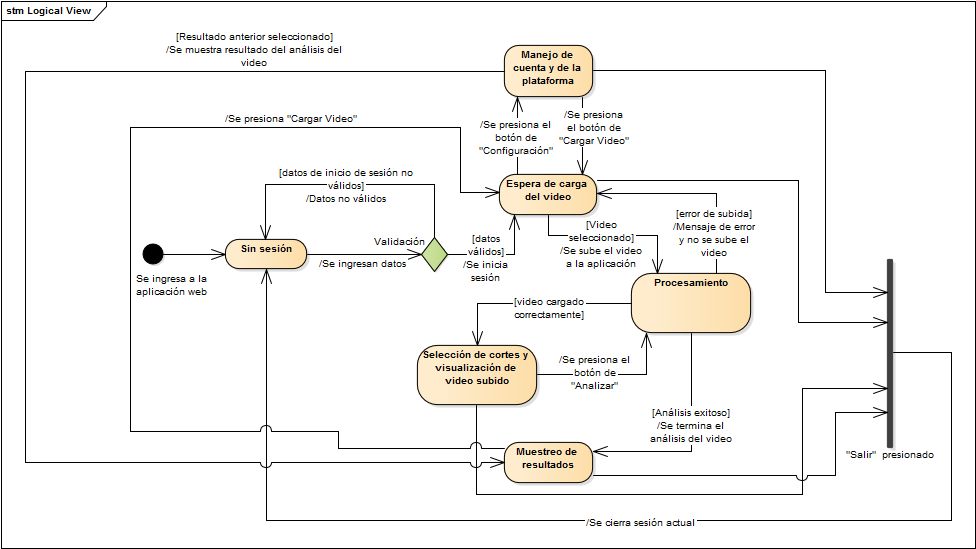
\includegraphics[width=1\linewidth]{Diagrama_estados.png}
  \caption{Diagrama de estados }
  \label{fig:State diagram}
\end{figure}  


\color{Blue}
\subsection{Características físicas}
\color{black}
\justify 

	\tab Las características físicas del producto se describen a continuación. 

\subsubsection{Requerimientos físicos} 

	\tab El sistema debe estar hospedado en una ubicación con acceso a internet las 24 hrs al día de forma que el servidor se conecte de forma indiferente a los clientes que entren a usar el sistema en todo momento. Como el uso de la aplicación es limitado a pocos usuarios inicialmente y luego a pocos usuarios que podrían darle uso distinto a la aplicación, la disponibilidad no debe ser absoluta y no debe ser reemplazable en caso de fallas en un tiempo menor al especificado en la sección 3.8.2.  El sistema estará hosteado en un servidor de Amazon Web Services.

\subsubsection{Requerimientos de adaptabilidad}

	\tab El sistema se estima que en un futuro podría integrarse como un módulo de un sistema de trabajo de videos para encontrar patrones o analisis extensivo de información en grandes cantidades. Así, se considera que deben ser completamente intercambiables las funciones que analizan los archivos de video así como aquellas que generan las estadísticas y datos de valor respecto al contenido analizado. 

\color{Blue}
\subsection{Condiciones de ambiente}
\color{black}
\justify 

	\tab Debido a que el servicio de hosting será brindado mediante  Amazon Web Services. Por este motivo, se exime de toda responsabilidad respecto a las condiciones ambientales del servidor al equipo original de desarrollo y se le delegan a la compañía externa mediante la obtención de sus servicios. 

\color{Blue}
\subsection{Seguridad del sistema}
\color{black}
\justify 

	\tab El sistema debe de validar el acceso de cada usuario mediante un sistema de \textit{Log In}, el cual tendrá una validación única mediante el nombre de usuario y una contraseña asociada a dicha cuenta. Esto se debe a que el sistema almacenará datos importantes acerca del rendimiento histórico de los jugadores en los partidos anteriores, lo cual podría ser considerado como información valiosa que debe mantenerse confidencial. \\

 El almacenaje de las cuentas se dará por parte del departamento de TI (\textit{Tecnologías de Información}) con una base de datos que ellos poseen y administran, por lo que la seguridad de estas cuentas. Esto se explicará más adelante en la sección 3.18 \textbf{Dependencias y Supuestos}.   Adicional a este requerimiento de seguridad, ningún otro requerimiento adicional fue solicitado por el cliente. Se exime de la integridad física del edificio en el que se encuentra el servidor del hosting como de la base de datos al equipo de desarrollo, ya que, como se explicó en el apartado anterior, son responsabilidades delegadas a la compañía externa. \\ \\
 
 
\color{Blue}
\subsection{Administración de la información}
\color{black}
\justify 

	\tab El sistema recibirá únicamente archivos de video, entre los que se permitirán archivos de extensión .mp4, avi, wmv, entre otros. Adicional a este tipo de archivos, se le permitirá también el registro de archivos .txt, .xml o .json como forma de archivos \textit{ground truth} para la segmentación temporal manual del video. Todos estos tipos de archivos pueden ser fácilmente ingresados al sistema mediante la aplicación web. \\ 
    
    El componente del servidor, que devolverá  directamente  archivos de video en formato .avi, los cuales vendrán a representar las escenas del video, también podrá devolver archivos contenedores de información. Estos últimos archivos contendrán los informes generados y podrán ser generados como .csv, .xml, .json o .txt. La información atómica de estos informes será almacenada en la base de datos de forma más unitaria, pudiendo estar en distintas tablas a través de distintos esquemas. Durante el desarrollo del sistema se podrán añadir nuevos requerimientos que requieran manejo adicional de la información, por lo que esta sección puede actualizarse. \\ \\

\color{Blue}
\subsection{Regulaciones y políticas}
\color{black}
\justify 

	\tab La plataforma web estará disponible en dos idiomas, siendo estos el inglés y el español. Puesto que el contrato es para un club de fútbol argentino, se seguirán conceptos y regulaciones establecidas por la FIFA para la delimitación y segmentación del campo, así como demás métricas y restricciones establecidas en los reglamentos acordes.  \\
    
    Se requerirá que cada cuenta esté asociada a un miembro del cuerpo técnico del club como de la junta administrativa, por lo que dichos datos serán requeridos a la hora de ingresar una cuenta y validados por el equipo de soporte del sistema. Estos datos serán albergados en la base de datos de manera encriptada, por lo que permancerán seguros a posibles filtraciones o robos de información. Adicional a estas regulaciones ninguna otra política es requerida por parte del equipo de desarrollo como del club Boca Juniors. \\ \\

\color{Blue}
\subsection{Sostenibilidad del ciclo de vida del sistema}
\color{black}
\justify 

	\tab Se establecerá la metodología ágil SCRUM para realizar un proceso de desarrollo de proyecto dinámico y ordenado, con el motivo de obtener la mejor calidad de software posible. En esta metodología se irán realizando sprints o iteraciones de desarrollo donde se trata de dejar en el mejor estado posible un componente entregable. Este componente será diseñado, programado y probado durante cada sprint. La metodología SCRUM dictamina la elaboración de reuniones al final de cada sprint llamadas Retrospectivas. Esto con el fin de extraer datos útiles de cada miembro del equipo y establecer o alterar objetivos y el rumbo general del proyecto.  \\
    
    También se asegurará que los desarrolladores reciban el proceso de capacitación apropíado para el manejo de las bibliotecas necesarias de análisis de video y \textit{computer vision.} Esto implicará el pago de un curso en plataformas educativas tales como \textit{edX} y \textit{coursera.} Los desarrolladores tienen la opción de tomar estos cursos o no, pero se les impulsa a tomarlos para disminuir el tiempo de la curva de aprendizaje y obtener un resultado más eficiente. \\
    
    Como actividad de aseguramiento de la calidad del software, se establecerán estándares de codificación para los lenguajes utilizados mayoritariamente, que en este proyecto son Java y Javascript. Los estándares escogidos fueron Google Java Style y el estándar determinado del verificador online \textrm{jshint}. Estos estándares facilitarán el mantenimiento de la herramienta y extenderá la vida del producto final.\\
    
    También se realizará una verificación de los requerimientos, diseño conforme a los requerimientos y código respecto al diseño al final de cada iteración del desarrollo. Se le consultará al cliente al realizar un cambio en el diseño de alto nivel o cualquier duda respecto a los requerimientos, siempre al final de una iteración o sprint. Estos procesos serán acorde al objetivo establecido en el  estándar IEEE-730, aunque no se seguirá este estándar al pie de letra. \\ \\


\color{Blue}
\subsection{Empaquetado, manejo, envío y transporte}
\color{black}
\justify 

	\tab Dado que el sistema se accede mediante una aplicación web y no es siquiera un bien físico, este sección será completamente omitida. Se asume que el cliente final ya posee una terminal con un navegador web y acceso a Internet, tal y como se especifica más adelante en la sección 3.18.  \\ \\

\color{Blue}
\subsection{Verificación}
\color{black}
\justify 

	\tab La verificación de los componentes se logrará mediante pruebas al final de cada iteración o etapa del desarrollo. Se recuerda que se utilizará SCRUM como metodología de trabajo y que esto requiere la realización de sprints iterativos. Tras cada sprint se utilizará la herramienta JUnit para la realización de test unitarios, en los componentes programados en JAVA, y de integración con los componentes web. \\
    
    Las pruebas de aceptación serán realizadas emulando los casos de uso en el que podrá estar el usuario al utilizar el sistema en su totalidad. Así, un miembro del equipo de desarrollo emulará dicho caso y ejecutará todas las funcionalidades de la misma manera de la que lo haría un usuario promedio. Si todo el proceso es exitoso, se considera que la prueba fue validada. \\ \\

\color{Blue}
\subsection{Dependencias y supuestos}
\color{black}  %%AÑADIR DATOS DE SEGURIDAD AQUÍ. 
\justify 

	\tab Para la correcta aplicación del sistema se asume que el usuario, grupo que como ya se ha mencionado varias veces, consistirá inicialmente de los miembros del cuerpo técnico del club Boca Juniors y de la Junta Administrativa de dicha agrupación;  presenta un navegador de internet que soporte Javascript y una conexión a Internet mayor a 512Kb/s. Factores adicionales como el sistema operativo de la terminal del cliente no son importantes en este proyecto ya que se accede al sistema mediante la aplicación web. \\
    
    A nivel del servidor se asume que los servicios brindados por AWS se integrarán sin problemas a los datos albergados en el hosting. Problemas con esta integración no serán responsabilidad del equipo de desarrollo al ser delegadas mediante\textit{outsourcing}. \\
    
    Respecto al almacenaje de las cuentas, esto será delegado al Club Boca Juniors mediante la Intranet que está bajo su propiedad. Esta base de datos almacena tablas con la información de los miembros pertenecientes al club y datos de la cuenta de estos miembros, así como los informes de los videos generados enlazados a cada usuario. Se supone que esta base de datos será actualizada y recibirá mantenimiento externo al del equipo de desarrollo. Mediante un componente de conexión, los datos de inicio de sesión serán obtenidos de esta base de datos. La seguridad así como la integridad de los datos se le delega al departamento de TI del Boca Juniors. 


\newpage
\color{Blue}
%\centering{ \rule{16cm}{0.1cm} }\\ 
\section{\textbf{Estándares de Codificación}}
\color{black}
\justify 

\tab En avances anteriores, se habían escogido dos estándares de codificación para el presente proyecto. Estos estándares eran el estándar de codificación planteado por Google para el lenguaje java llamado \textit{Google Java Style} y el estándar de codificación para javascript brindado por la herramienta en línea \textbf{jshint.com}. Estos dos estándares han sido implementados en el código fuente del proyecto desde entonces, siendo el estándar de Java implementado automáticamente mediante la herramienta o \textit{plugin} de Eclipse \textbf{CheckStyle}. A continuación, se muestra un tutorial sobre cómo instalar y utilizar esta herramienta para automatizar la conformidad del estándar en el proyecto. 

\color{Blue}
\subsection{Herramienta de verificación CheckStyle.}
\color{black}

\textit{Checkstyle} es una herramienta automatizada de revisión de código estático, especial para entornos en donde se utiliza el lenguaje Java. Permite a los programadores revisar si su código java se adhiere a un estándar específico, entre los cuales tiene como opciones predeterminadas al estándar de codificación de \textit{Sun Code Conventions} y el \textit{Google Java Style}, el cual es el elegido en este caso. El método para instalación de esta herramienta y su utilización en el entorno de desarrollo Eclipse se explica a continuación:
    
    
\begin{itemize}
\item Al tener el entorno de desarrollo abierto, diríjase a la pestaña \textbf{Help} o \textbf{Ayuda}, en la parte superior de la ventana y seleccione la opción \textbf{Eclipse MarketPlace}. La imagen muestra la localización de esta opción.
\end{itemize} 
\centering
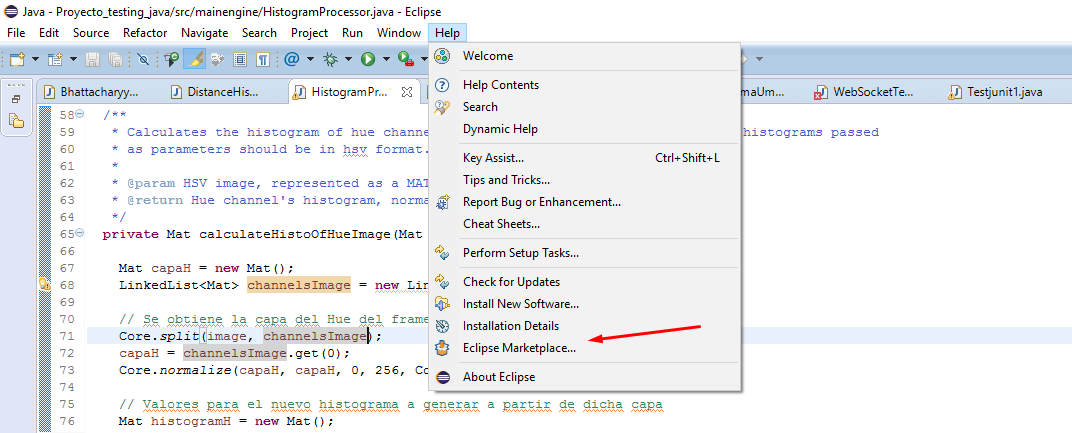
\includegraphics[scale=0.5]{Screenshot_CheckStyle_1.png}
\justify
\begin{itemize}
\item Al abrirse la ventana, diríjase a la ventana \textbf{Search} e introduzca \textit{Checkstyle} en el espacio de búsqueda. Podrá ver que el buscador lanzará como resultado el \textbf{Checkstyle Plug-in}. Seleccione el botón de Instalar y siga el proceso de instalación, el cual le pedirá reiniciar Eclipse al finalizar. En la imagen se muestra la pestaña de \textbf{Installed} y el botón de \textbf{Uninstall} en vez del de \textbf{Install} al estar el plugin ya instalado en la terminal. Si lanza una ventana de advertencia durante el proceso de instalación diciendo que se está instalando software de fuentes desconocidas, proceda a ignorar esta advertencia. 
\end{itemize} 
\centering
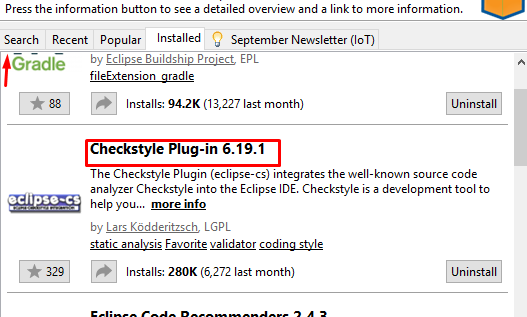
\includegraphics[scale=0.5]{Screenshot_CheckStyle_2.png}
\justify
\begin{itemize}
\item Tras reiniciar Eclipse, deberíamos contar con la herramienta de Eclipse ya instalada en nuestro entorno local de desarrollo. Ahora basta activarlo en el proyecto para poder utilizarla. Para hacer esto diríjase al \textit{Project Explorer} y realice click derecho sobre el proyecto, el cual debería estar en el \textit{Workspace} para este momento. Diríjase al botón \textbf{Properties}, tal y como indica la imagen.
\end{itemize} 
\centering
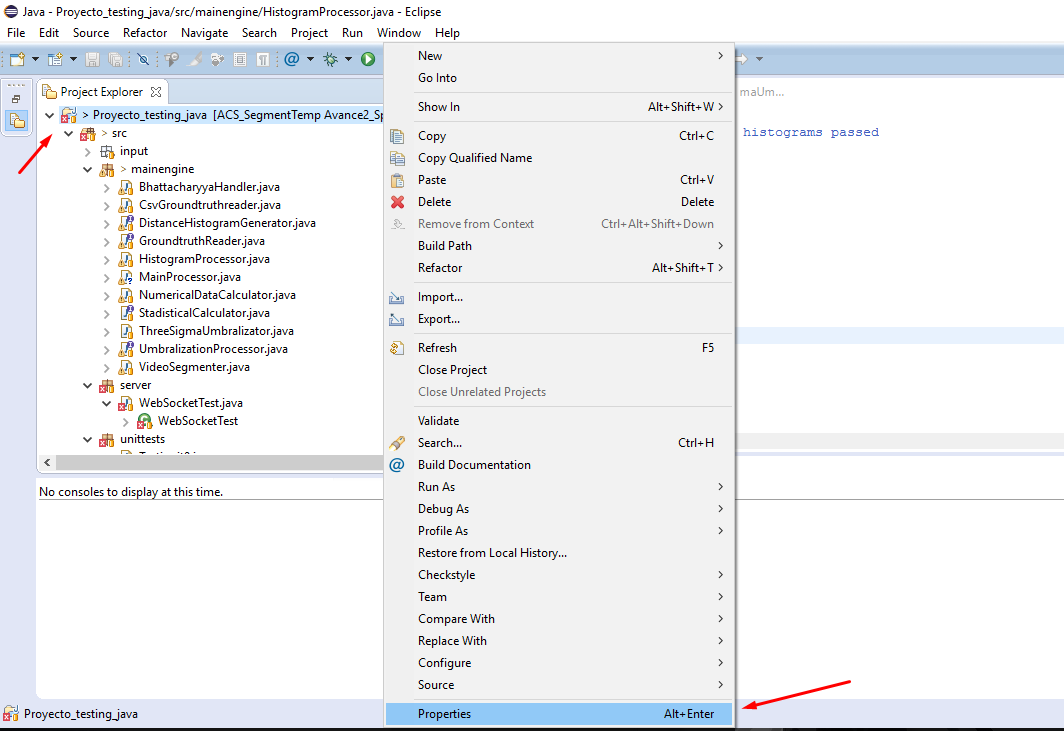
\includegraphics[scale=0.5]{Screenshot_CheckStyle_3.png}
\justify
\begin{itemize}
\item En la barra lateral, asegúrese de entrar al menú de \textbf{CheckStyle} y una vez dentro, active la opción \textbf{Checkstyle active for this project.} Esto debería permitir utilizar la herramienta en el proyecto. La imagen indica la posición de estas opciones. Asegúrese de que el estándar de Google o \textit{Google Checks} esté activado en el \textit{combobox} de \textbf{Check Configuration}.
\end{itemize} 
\centering
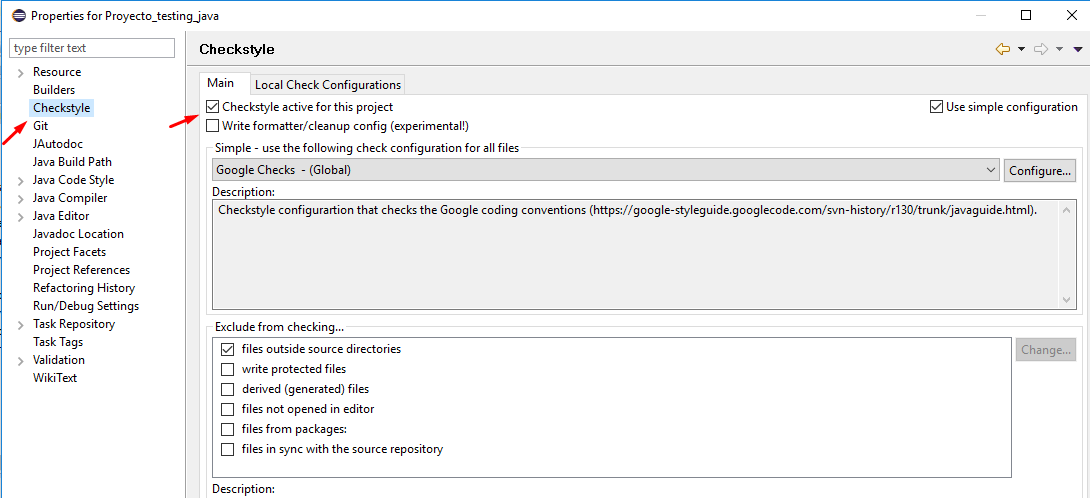
\includegraphics[scale=0.5]{Screenshot_CheckStyle_4.png}
\justify
\begin{itemize}
\item Para poder utilizar la herramienta de CheckStyle, seleccione click derecho en el \textit{Project Explorer} los archivos de código fuente que desea verificar y en la opción de \textbf{CheckStyle}, haga click sobre \textbf{Check code with CheckStyle}. Esto debería activar un chequeo de implementación del estándar seleccionado.
\end{itemize} 
\centering
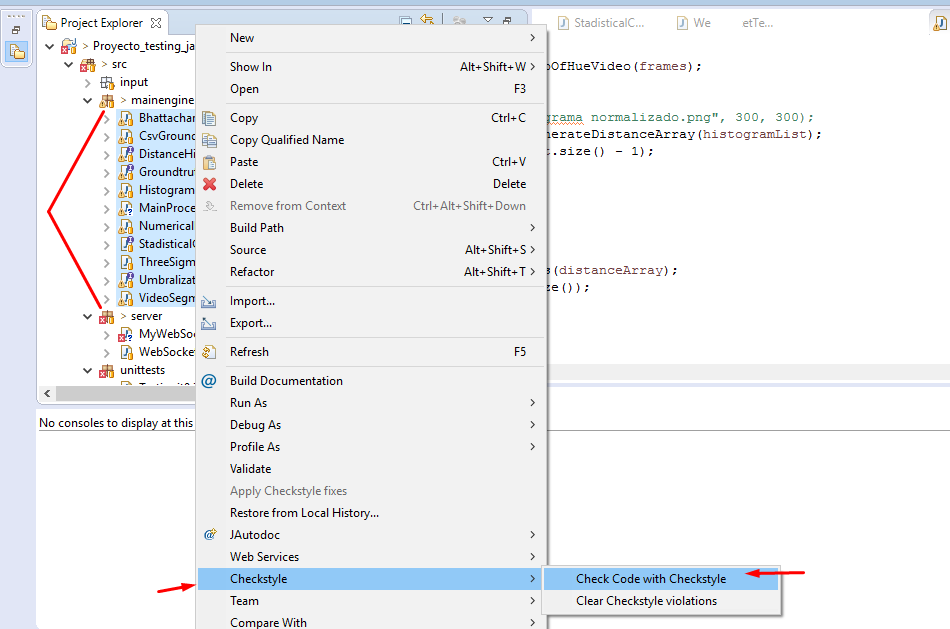
\includegraphics[scale=0.5]{Screenshot_CheckStyle_5.png}
\justify
\begin{itemize}
\item Dicho chequeo mostraría con una lupa al lado izquierdo del editor de texto del entorno de desarrollo Eclipse aquellas líneas del archivo de código fuente que cuenten con violaciones al estándar de codificación \textit{Google Java Style}. Al mantener el cursor sobre dicho símbolo, un \textit{tooltip} mostrando el tipo de violación específica aparecerá. Todo esto se muestra en la siguiente imagen.
\end{itemize} 
\centering
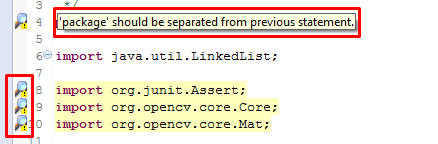
\includegraphics[scale=0.8]{Screenshot_CheckStyle_6.png}
\justify
\begin{itemize}
\item CheckStyle es una herramienta únicamente de verificación, lo que indica que únicamente revisará el código, mas no lo corregirá. Eclipse cuenta con un formateador de código, siguiendo una configuración específica. Como punto extra a este tutorial, se enseñará a corregir de manera automática y rápida el código para que siga el estándar de codificación. Diríjase otra vez a las propiedades del proyecto haciendo click derecho sobre la carpeta del proyecto en el \textbf{Project Explorer} y seleccionando la opción  \textbf{Properties}. 
\item Al abrirse la ventana de propiedades del proyecto, diríjase al menú \textbf{Java Code Style} y de ahí al submenú \textbf{Formatter}. En la carpeta raíz del repositorio debería haber un archivo llamado \textbf{\url{eclipse-java-google-style.xml}}. Asegúrese de que exista y que se encuentre en la copia local de su repositorio. 
\item Seleccione el botón de configuración \textbf{Configure Workspace Settings}. La posición del botón es mostrado en la siguiente imagen.
\end{itemize} 
\centering
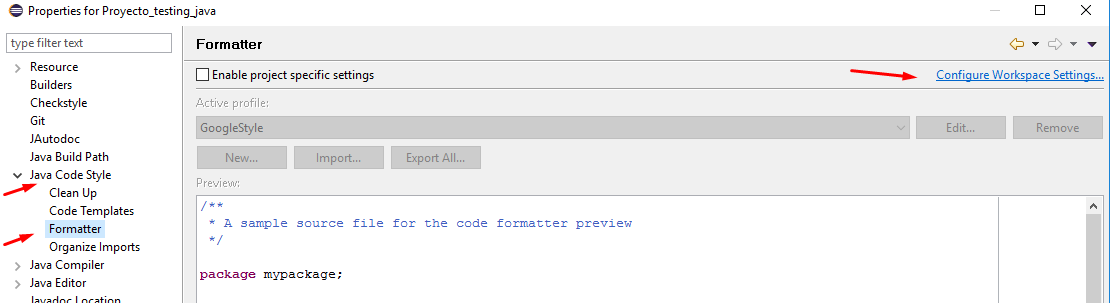
\includegraphics[scale=0.5]{Screenshot_CheckStyle_7.png}
\justify
\begin{itemize}
\item Al abrirse la ventana, seleccione el botón de \textbf{Import} y seleccione el archivo .xml anteriormente referenciado. La imagen muestra la posición del botón. Una vez seleccionado dicho archivo y configurado el tipo de formateo de código al de \textit{Google Java Style}, puede seleccionar el código en el editor de texto y presionar Ctrl$+$Shift$+$F.
\end{itemize} 
\centering
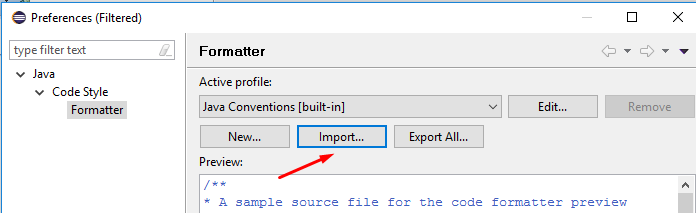
\includegraphics[scale=0.5]{Screenshot_CheckStyle_9.png}
\justify


\justify 
\newpage
\color{Blue}
\centering{ \rule{16cm}{0.1cm} } 
\justify 
\color{Blue}
\section{Validación del diseño}
\color{black}
\justify 

\tab En la siguiente tabla se muestran las relaciones entre las unidades de diseño y los requerimientos del sistema:\\
    
\begin{table}[h!]
\begin{tabularx}{\textwidth}{|p{5cm}|p{9.1cm}|}
\hline
  \textbf{Artefacto de diseño}& 
  \textbf{Requerimientos asociados}\\

  \hline
  Diagrama de Casos de Uso&
  Los requerimientos funcionales relacionados son.
  \begin{itemize}
\item 1.4.1 de acceso a la aplicación.     
\item 1.4.2 para la subida del video (las opciones que tiene el  usuario y lo que debe presentársele).     
\item 1.4.3 de envío del video para análisis pues muestra las opciones que tiene el usuario para iniciar el proceso de análisis). 
\item 1.4.6 por los subrequerimientos 1.4.6.2, 1.4.6.3, 1.4.6.4, 1.4.6.5.     
\item El requerimiento 1.4.7 por las opciones que tiene el usuario para subir el ground truth en la interfaz.     
\item 1.4.8 por la presentación de la información del ground truth (1.4.8.1) 
  \end{itemize} 
  
  Los requerimientos de usabilidad 1.5 están relacionados seriamente con los casos de uso por definición. 
  
\\
  \hline
  Diagrama de Clases&
  Inverso a los requerimientos relacionados al diagrama de casos de uso, estos se enfocan más en el código del servidor y los procesos internos del programa, por lo que se relaciona a los requerimientos funcionales: 		
  \begin{itemize}
\item 1.4.3.3 y 1.4.3.4 por el manejo de errores y del tiempo de ejecución. 
\item 1.4.4 por el servidor pues se encarga de muestrear la forma en la que se relaciona con el resto de clases. 
\item 1.4.5 y todos sus subrequerimientos: 1.4.5.1 por la implementación del Bhattacharyya y 1.4.5.2 por el teorema de los tres sigmas pues muestra una forma inicial de cómo es que se implementa. \item 1.4.6 porque se muestra la forma inicial en la que se obtienen los resultados.
  \end{itemize} 
  
  Pueden mapearse también a los requerimientos de eficiencia 1.6 en caso de que se quiera hacer un análisis particular de algún elemento o relación. 
\\

  \hline
  \end{tabularx}
\caption*{\color{Red} \color{Black}}
\end{table}

\newpage
\begin{table}[h!]
\begin{tabularx}{\textwidth}{|p{5cm}|p{9.1cm}|}
\hline
  Diagrama de Componentes&
  Los requerimientos funcionales asociados son:
  \begin{itemize}
  \item 1.4.2 porque se muestra el proceso por el que pasan los videos que son subidos. Específicamente al requerimiento 1.4.2.3
  \item 1.4.4 porque se muestran de forma específica cuáles son los componentes relacionados al servidor y de qué forma se relacionan con los componentes del front end. 
  \item 1.4.6 pues da una idea general de la forma en que se relacionan los componentes para devolver los resultados y que se puedan presentar en el front end. 
  \item 1.4.7 pues se muestra o se da una idea, al igual que en la 1.4.2, cómo viaja el ground truth entre componentes. 
  \end{itemize} 
  Se relaciona hasta cierto punto a los requerimientos de eficiencia pues los componentes pueden ser analizados individualmente en búsqueda de mejoras de eficiencia particulares. \\
  
  \hline 
  Diagrama de Actividad&
  Los requerimientos funcionales asociados son:
  \begin{itemize}
  \item 1.4.2, específicamente a 1.4.2.1 y 1.4.2.4 pues son la interacción que tendrá el usuario con el sistema. También relacionado está 1.4.2.5 por el muestreo de errores. 
  \item 1.4.3, especialmente por la 1.4.3.1 porque se muestra la opción con la que ha de interactuar el usuario para enviar el video, y los errores que puede recibir (1.4.3.4)
  \item 1.4.6, enfocado en 1.4.6.2, 1.4.6.3, 1.4.6.4 porque es la interacción resultado para que el usuario vea lo que resolvió el sistema. 
  \item Es una tarea por sí misma relacionada también a 1.4.6, el requerimiento 1.4.6.5 muestra como el sistema debe permitir la interacción para obtener el archivo con los resultados. 
  \item 1.4.7, con 1.4.7.1 pues es la interacción mediante la cual el usuario sube un video al sistema. 
  \item 1.4.8, en especial de 1.4.8.1 para presentar el análisis comparativo. 
  \end{itemize}
  Los requerimientos de usabilidad 1.5 están relacionados a este diagrama pues muestra la forma en que la actividad del usuario respecto al sistema. \\
    \hline
  
\end{tabularx}
\caption*{\color{Red} \color{Black}}
\end{table}

\newpage
\begin{table}[h!]
\begin{tabularx}{\textwidth}{|p{5cm}|p{9.1cm}|}
  
  \hline
  Diagrama de Estados&
    Los requerimientos funcionales asociados son:
  \begin{itemize}
  \item Está relacionado de forma general a los requerimientos funcionales 1.4, porque el diagrama de estados permite visualizar la forma en la que los requerimientos se relacionan entre sí. 
  \item Además se relaciona generalmente a varios requerimientos de usabilidad 1.5 pues muestra la forma en que el sistema reaccionará de acuerdo al uso que se le dé. 
  \end{itemize}\\ 
  \hline
\end{tabularx}
\caption*{\color{Red} \color{Black}}
\end{table}
  


\newpage
\color{Blue}
\centering{ \rule{16cm}{0.1cm} } 
\justify 
\subsection{\textbf{Jenkins: Tutorial de configuración}}
\color{black}

\justify 

\tab Jenkins es una herramienta de integración continua, que proviene de Hudson (es un fork de dicho proyecto) y que propone un sistema de fácil instalación y configuración. La portabilidad de esta herramienta representa un problema pues está pensada para Linux principalmente. La configuración en primer instancia debería ser sencilla en cualquier sistema operativo, pero por una situación con la generación de credenciales para el usuario de Jenkins, en Windows no fue posible configurarlo sin abrir una máquina virtual con un servidor de ubuntu y una referencia desde el servicio de Jenkins en Windows. Como esto es inacceptable y un verdadero desastre, para este tutorial, se muestra una versión únicamente para Ubuntu 16.04, en donde la dimensión del problema sigue siendo tolerable. 

1. Primero, descargar Jenkins del sitio oficial: 
\url {http://pkg.jenkins-ci.org/debian-stable/} , en esta misma página encontrará instrucciones para descargar desde la terminal. Estas son: 
	\begin{itemize}
    \item Ejecutar el primer comando: \textbf{ wget -q -O - https://pkg.jenkins.io/debian-stable/jenkins.io.key | sudo apt-key add -}
    \item Ejecutar \textbf{sudo nano /etc/apt/sources.list} Nano es un editor de texto en consola que abrirá el archivo sources.list en esa ubicación. 
    \item A ese archivo, agregar el comando \textbf{ deb https://pkg.jenkins.io/debian-stable binary/ } al final del archivo. 
    \item Ejecutar \textbf{sudo apt-get update} y 
\textbf {sudo apt-get install jenkins} para comenzar la instalación. 
    \end{itemize}
    
    De forma alterna (y recomendada), descargar la versión estable más reciente para instalación directa del .deb. 

\centering
	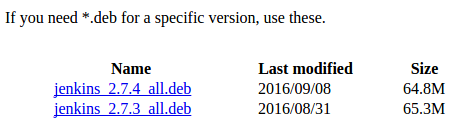
\includegraphics[scale=0.5]{jenkinsdeb}
\justify

\tab 	Y luego, desde la carpeta donde se descargó el .deb (click derecho Open Terminal), ejectuar 
    \begin{itemize}
    \item \textbf {sudo dpkg -i nombrepaquete (en este caso, jenkins\_version\_all.deb)}
	\item La interpretación del comando anterior es para nuestro ejemplo: \textbf{sudo dpkg -i jenkins\_2.7.4\_all.deb}
    \end{itemize}
    
    \textbf{En caso de que diera error por falta de un daemon, sudo apt-get -f install resolvería los problemas de la dependencia faltante.}\\
    
\newpage 2. En este punto, Jenkins fue descargado. Lo que sigue es instalarlo junto con los plugins requeridos para la inicialización de un proyecto con el repositorio. 
    
\centering
	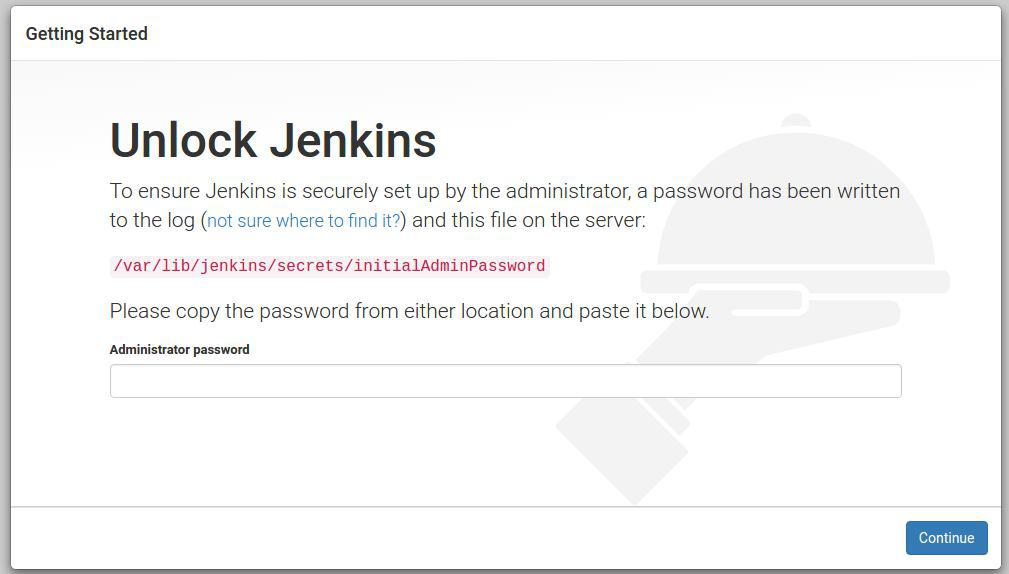
\includegraphics[scale=0.5]{unlockjenkins}
\justify

Si abre un browser (en este caso Google Chrome) y entra a localhost:8080, por defecto, el servicio de Jenkins corre en dicho puerto de localhost, le preguntará por una contraseña inicial. \\

	Puede ejecutar \textbf {sudo cat /var/lib/jenkins/initialAdminPassword} para obtener directamente el contenido del archivo texto con la llave, o puede abrir manualmente el archivo y recuperar el texto. Después de copiarlo y pegarlo, dé click en Continue. \\

	Una vez con acceso, le aparecerá esta opción. Escoja Install Suggested Plugins pues no hace falta complicarse de más. \\

\centering
	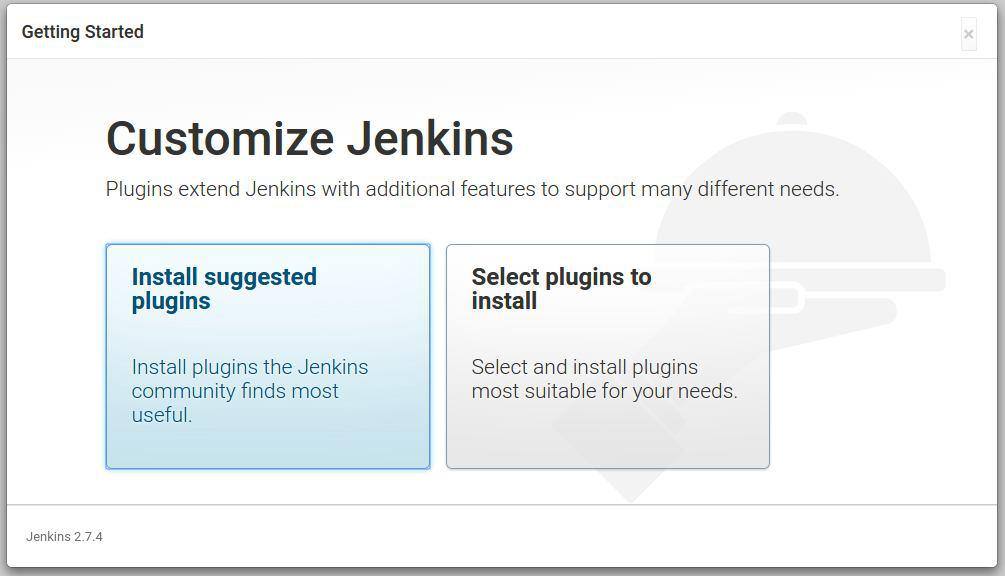
\includegraphics[scale=0.5]{suggjenkins}
\justify

\newpage Le aparecerá una pantalla como la siguiente. Espere a que se complete el proceso de instalación.  \\
   
\centering
	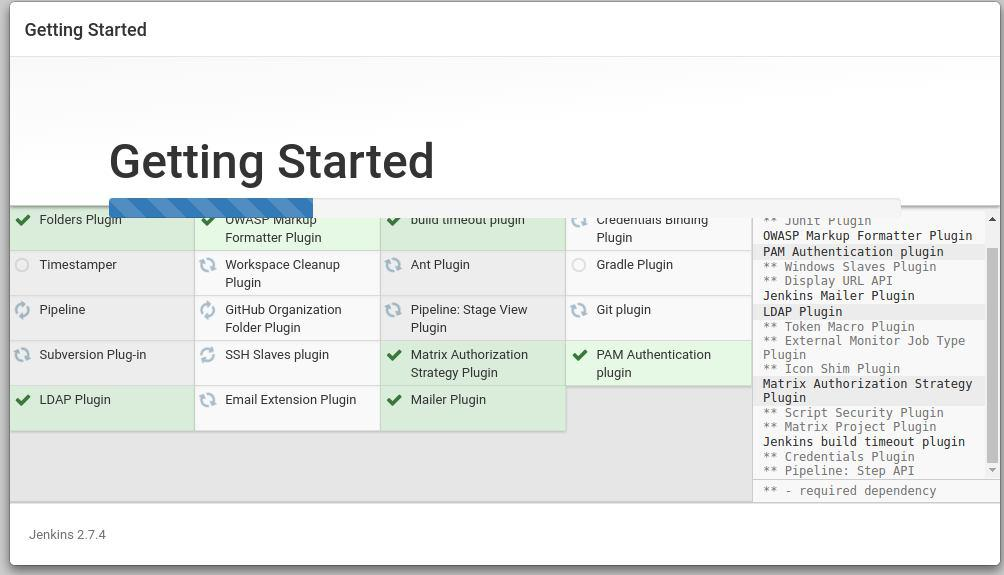
\includegraphics[scale=0.5]{progjenkins}
\justify
  
\tab La mayoría de tutoriales de fácil acceso en internet le indicarán la forma de instalar manualmente los plugins de Github y Git, sin embargo en la pantalla anterior se puede ver cómo ambos son plugins sugeridos para Jenkins (al menos, en la versión de este tutorial), por lo que no hará falta instalarlos de nuevo. \\

3. Ahora, configuraremos el usuario de uso de Jenkins. Este paso es vital pues Jenkins el resto del tutorial hará uso de estos datos, así que es recomendado tenerlos a mano. 

Para este tutorial, diremos que el usuario es \textbf{menoc} y el password es cualquier cadena. Llene los demás datos como es evidente que debe hacerse, y dé click en Save and Finish para continuar. Aparecerá esta pantalla diciendo que el proceso fue exitoso. \\

\centering
	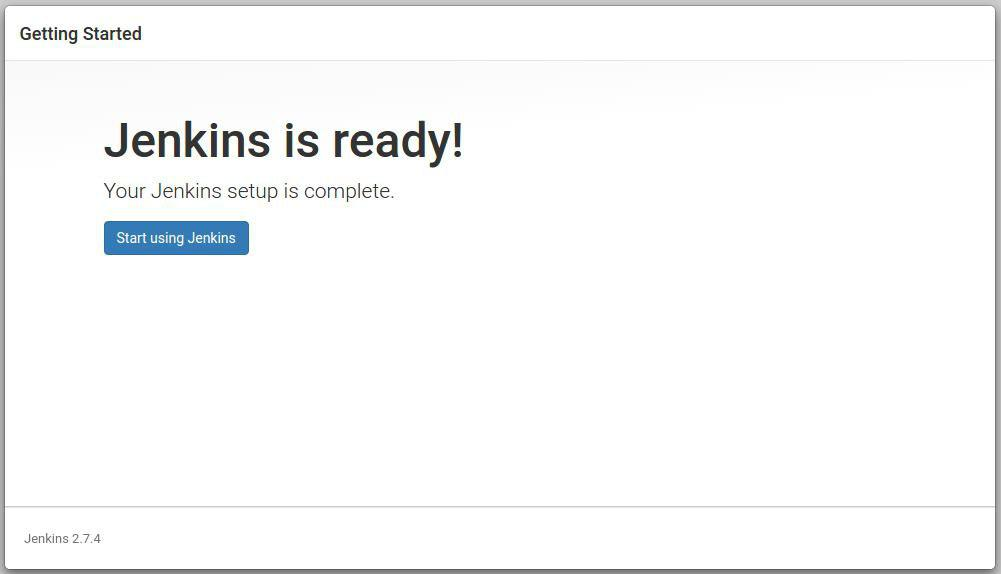
\includegraphics[scale=0.5]{jenkinsready}
\justify

Ahora, recargue o abra de nuevo Jenkins y obtendrá la sigueinte pantalla principal en la que deberá iniciar sesión con el usuario que acaba de crear. 

\centering
	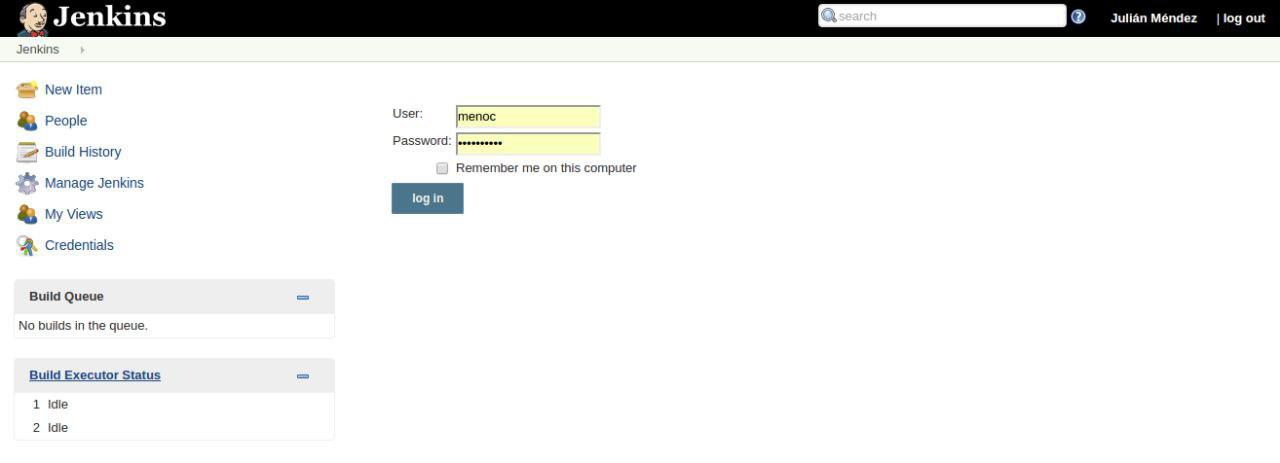
\includegraphics[scale=0.5]{maainjenkins}
\justify

Dé click en login y estamos listos. 


\centering
	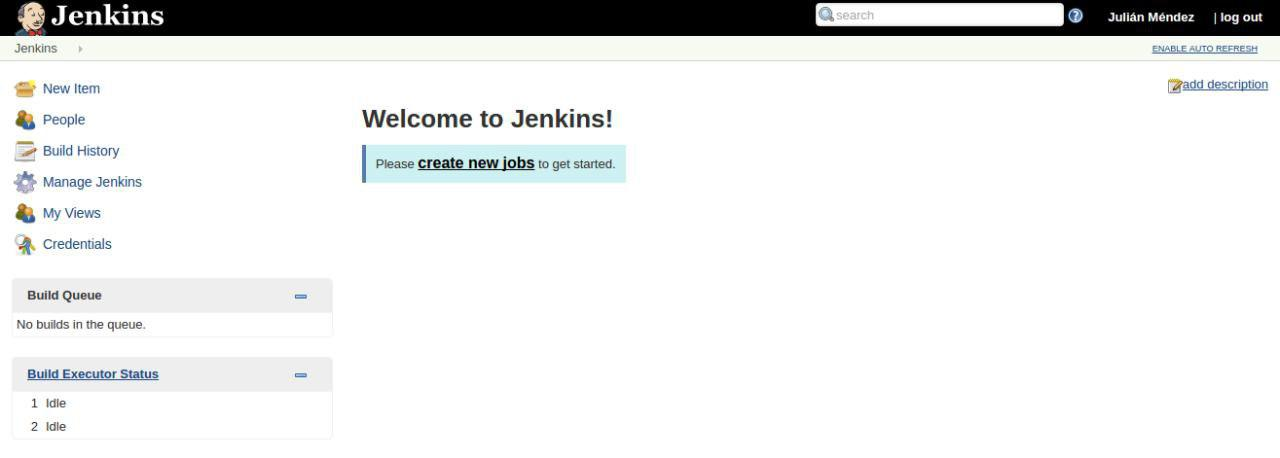
\includegraphics[scale=0.5]{jenkinsaskjob}
\justify

\newpage

4. Configurar el Item de Jenkins con el proyecto de Github\\

	En el último screenshot se mostraba al lado izquierdo la opción New Item. Dé click ahí para crear un nuevo Job. Como ya se dijo previamente, en la mayoría de tutoriales aparecen los pasos para instalar el plugin de Github y Git pero no hará falta. En caso de que estos plugins no estén instalados, debe entrarse a Manage Jenkins, Manage Plugins, buscar Github e instalarlo (traerá todos los plugins relacionados que requiere para funcionar). \\

\centering
	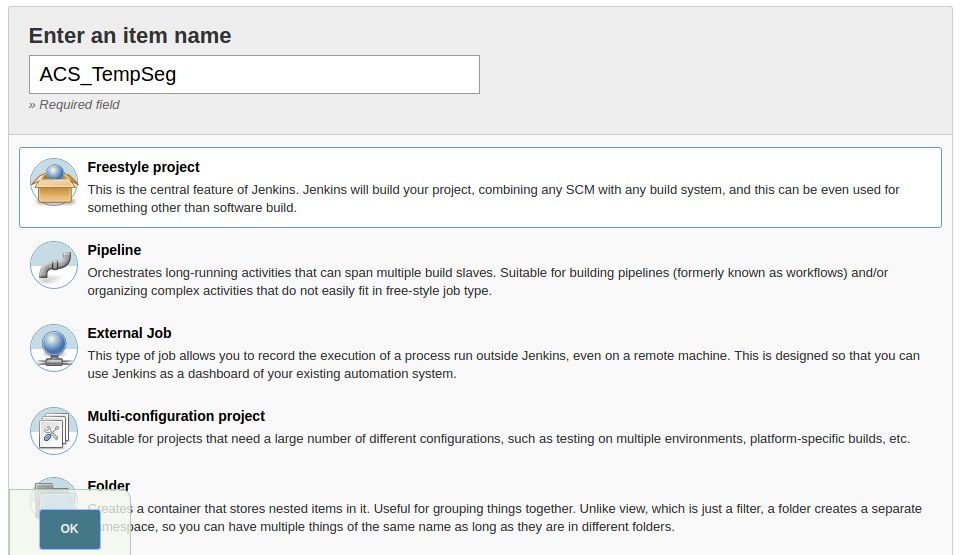
\includegraphics[scale=0.4]{newitem}
\justify

\tab Seleccione el nombre de su Job. En este caso, será ACS\_TempSeg por el motivo del proyecto. Después, seleccione Freestyle project y luego OK para continuar. \\

La siguiente parte es el motivo por el que se trabaja en Linux (Ubuntu 16.04 en este caso). 

Siga con cuidado los siguientes pasos pues algún fallo complicará de forma ridícula la instalación. 

	\begin{itemize}
    
    \item Abra la terminal y ejecute \textbf{sudo -i} para usar el usuario root
    \item Ejecute \textbf{apt-get install git -y}
    \item Ejecute \textbf{apt-get install apache2 -y}
    \item Ejecute \textbf{chown jenkins /var/www/html -Rf}
    \newpage
    \item Ejecute \textbf{visudo} lo que entrará a un editor de texto. \\
    	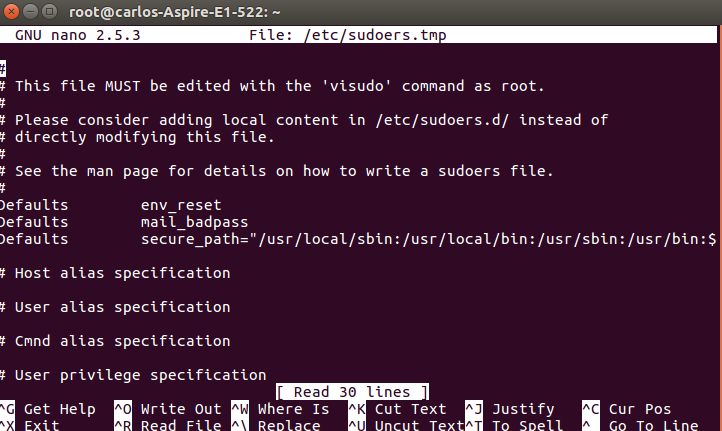
\includegraphics[scale=0.5]{visudo}
    \item Ubíquese en la línea debajo de Defaults secure\_path etc y escriba\\ \textbf{Defaults:jenkins !requiretty,!lecture}\\
\textbf{jenkins ALL=NOPASSWD:/etc/init.d/apache2}\\
    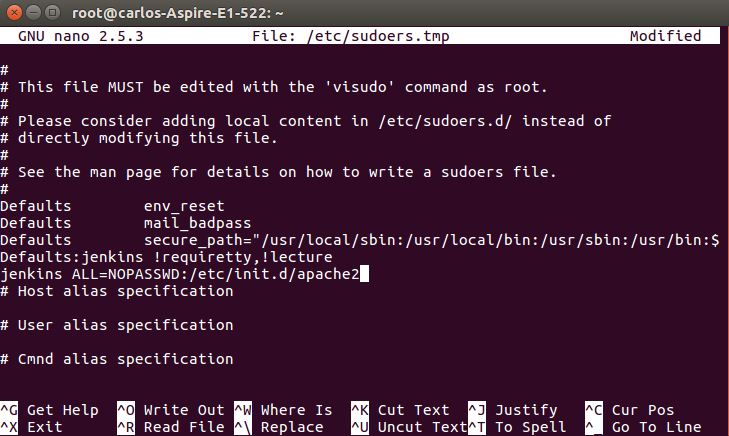
\includegraphics[scale=0.5]{visudo2}\\
	Salve el archivo con Ctrl + X, luego Y y por último Enter para confirmar. 
    \item Esto asegura que apache está instalado, da permiso a Jenkins de copiar archivos al directorio web y permite reiniciar fácilmente apache. 
    \item NO CIERRE ESTA TERMINAL AÚN. 
	\end{itemize}
    
    Ahora que todos esos pasos fueron correctamente ejecutados, es importante hacer la aclaración de que en un proyecto a gran escala, apache corre en un server aparte que es accesado. Todos los pasos anteriores son simplemente para poder conectar correctamente el repositorio de forma local. 
    
\newpage  
    Ahora, veamos cómo configurar el repositorio. Entre a github y copie el ssh del repositorio que desea configurar. \\
    
\centering
    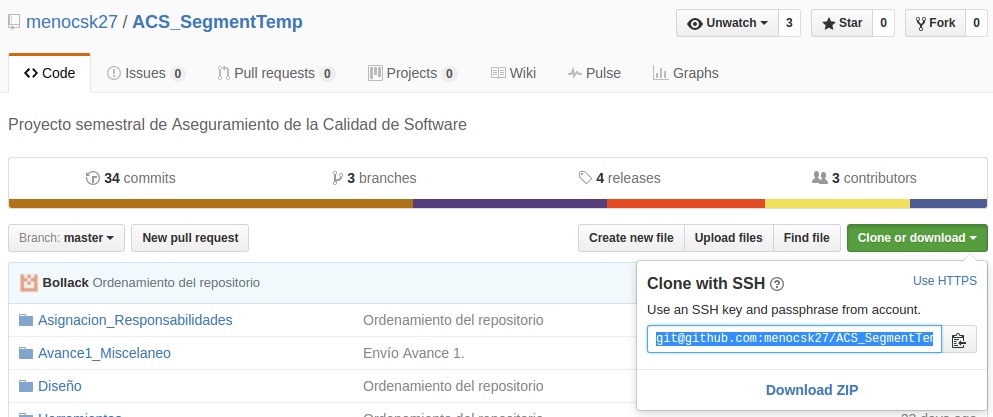
\includegraphics[scale=0.4]{repossh}\\
\justify

    En la terminal que estaba en root, haga lo siguiente. De nuevo, los siguientes pasos involucran comandos de terminal, por lo que debe tenerse cuidado. \\
    
    \begin{itemize}
    \item Ejecute \textbf {su jenkins} para cambiar al usuario de jenkins. 
    \item Ejecute \textbf{cd ~} para cambiar al directorio home de jenkins.   
    \item Ejecute \textbf {git clone git@github.com:menocsk27/ACS\_SegmentTemp.git} o el ssh que del repo que se quiere clonar. \\
    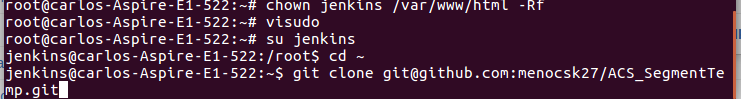
\includegraphics[scale=0.5]{git_clone.png}\\
	\item Aparecerá un mensaje de error y luego una solicitud de confirmación, escribimos \textbf{yes} y ahora github es uno de los hosts conocidos. \\
    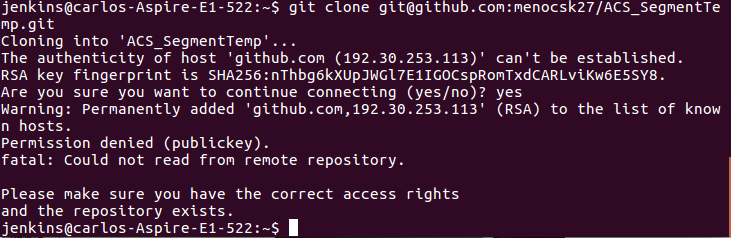
\includegraphics[scale=0.5]{permdenied}\\
	\end{itemize}
    
    \newpage En este punto nos aparecerió un mensaje de error diciendo que la conexión no puede activarse, pero eso está bien. Lo que haremos ahora es generar un llave SSH de acceso a github para obtener esos permisos. Lo último que haremos en la consola antes de volver a la interfaz de usuario de Jenkins es generar esa llave. 
    
    \begin{itemize}
    \item Ejecutamos \textbf{ssh-keygen -t rsa -b 4096 -C ''menoc.sk27@gmail.com''} Donde el correo electrónico es el correo relacionado a la cuenta de Github. Pedirá un par de cosas más pero con dar Enter basta. \\
        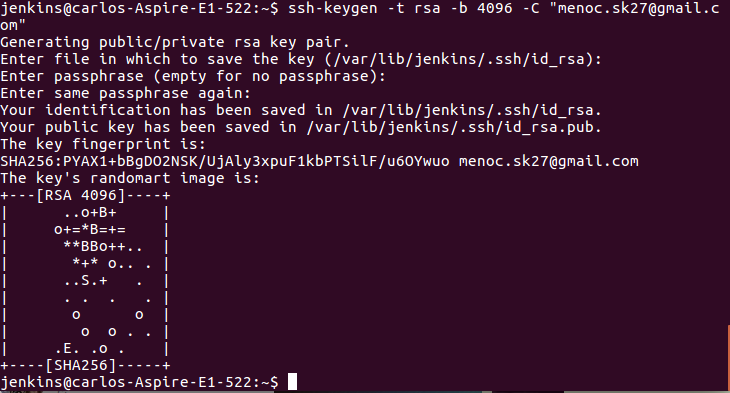
\includegraphics[scale=0.5]{sshkey}\\ 
    Con esto se generó la llave que usaremos para conectarnos al repositorio desde Jenkins
    \item Ejecute \textbf{cat ~/.ssh/id\_rsa.pub} y se mostrará la llave generada. \\
    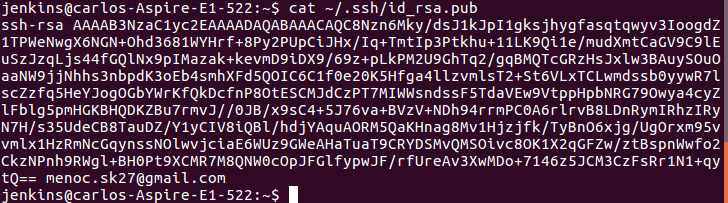
\includegraphics[scale=0.5]{llave}\\
    \item Copie todo eso al clipboard
    \item Entre a github en su cuenta $\rightarrow$ Settings\\
    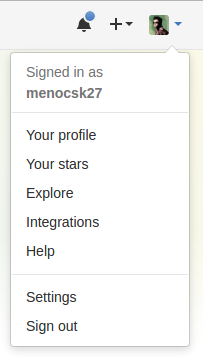
\includegraphics[scale=0.5]{gitset}\\
    \item Escoja SSH and GPG Keys, agregue una nueva con el nombre que guste y copie la llave que copió de la terminal.\\
    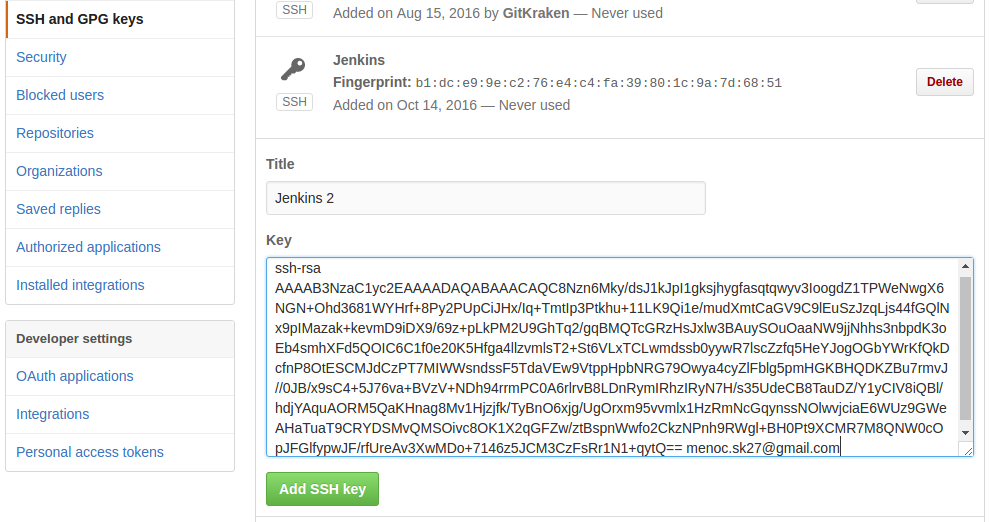
\includegraphics[scale=0.4]{sshkeygit}\\
    Luego, dé Add SSH Key para agregarla. 
    \item Ahora, el comando que antes dio error no lo dará. Sin embargo, esto no nos importa ya, porque cumplió su propósito de hacer que Jenkins conozca Git. 
    \end{itemize}
    
    Veamos ahora cómo configurar el control de versiones en la interfaz de Jenkins. 
    Estábamos aquí:
	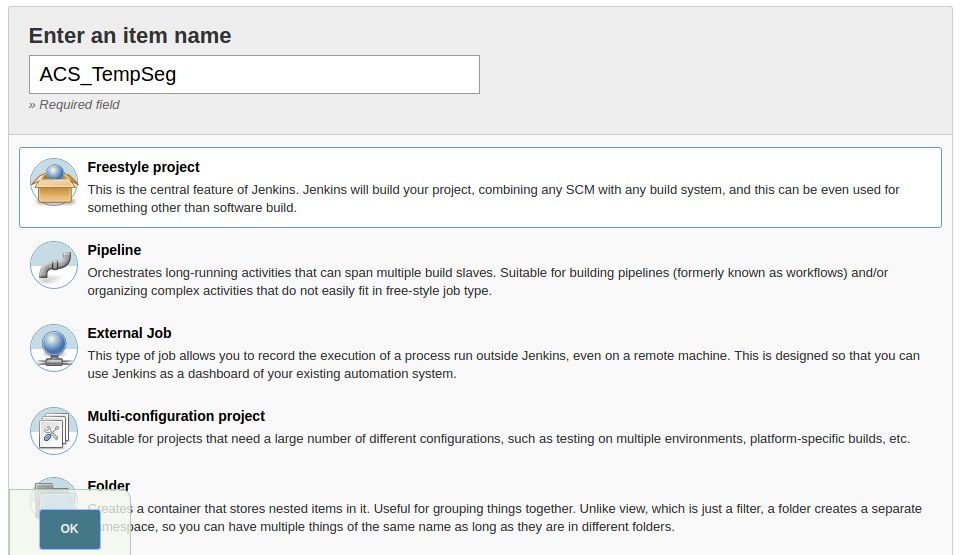
\includegraphics[scale=0.3]{newitem} y dimos ok. La pantalla que tenemos ahora es esta: 
    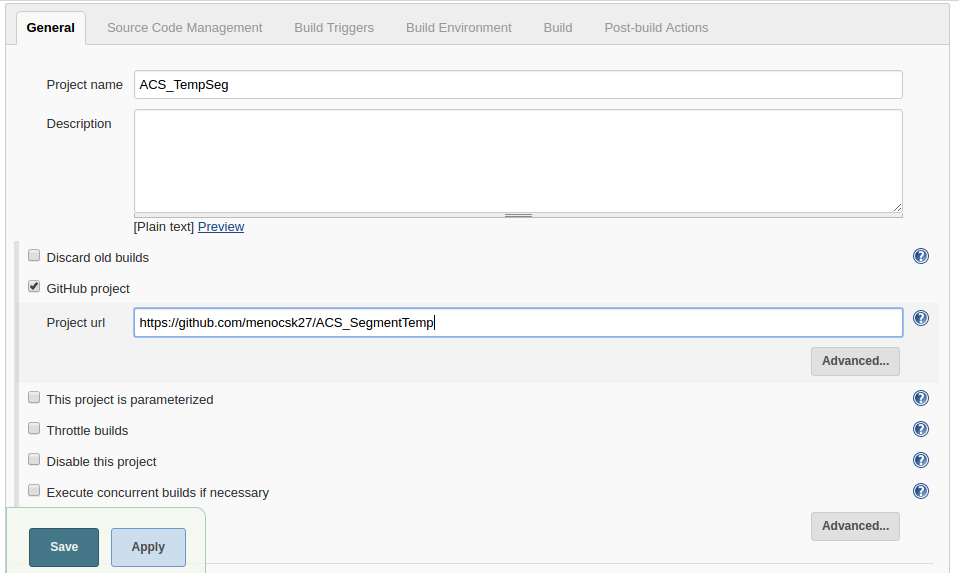
\includegraphics[scale=0.3]{sourcecontrolgitjenkins} Escogemos GitHub project y copiamos la dirección del repositorio, luego bajamos aquí:\\
   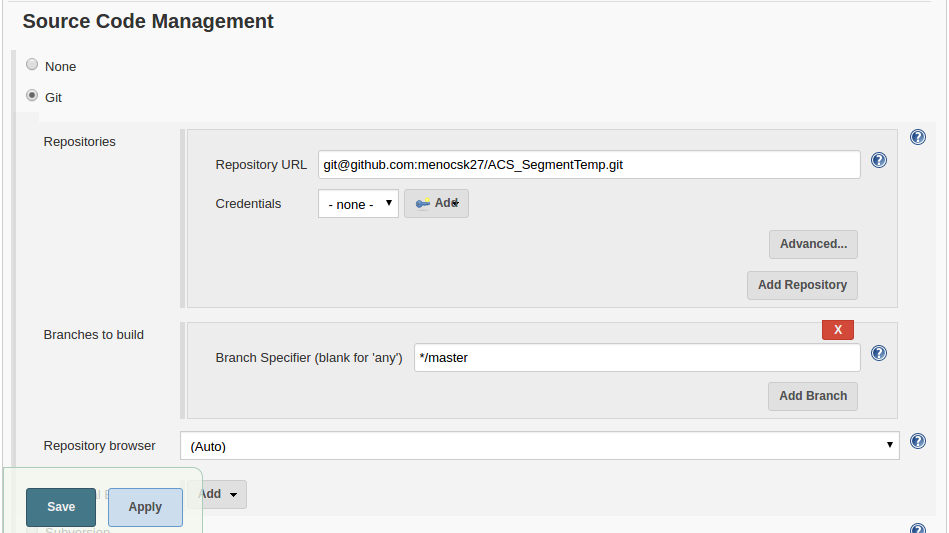
\includegraphics[scale=0.3]{repositorygitssh}\\
   
   Tras copiar ese SSH, si algo de lo anterior no salió, tirará un error que produce náuseas y tendencias suicidas. Pero si todo salió bien, no tira error y no tira nada anormal, dé click en Save. \\
   
   Jenkins ahora tiene un proyecto o Job configurado con la dirección de nuestro repositorio y está listo para ejecutar rutinas cada vez que se hace un commit. Ahora probaremos la ejecución de una rutina simple, para asegurarnos que todo salió como esperábamos. \\
   
   Volvamos a la página de configuración del proyecto dando click en Configure. Bajamos hasta las últimas opciones, en la de Build, damos click en Add build step y escogemos Execute Shell. Se abre un espacio para escribir el comando, donde haremos simplemente un echo. \\
   
      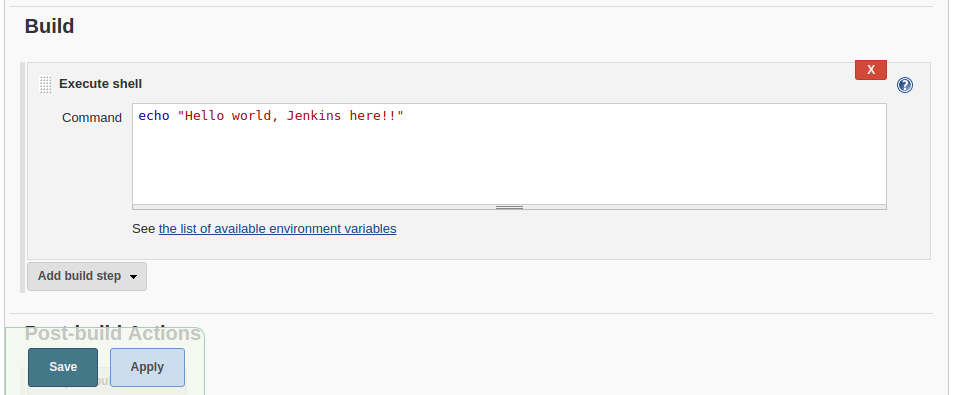
\includegraphics[scale=0.3]{hellojenkins}\\
   
   Damos Save una vez más.  
   
   
   \newpage 
   5. La gloria. \\
   
   En la ventana principal del Job del proyecto le damos Build Now. \\
      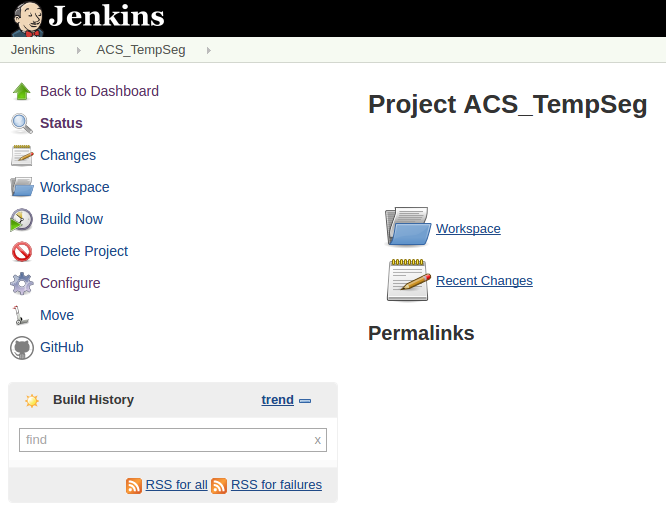
\includegraphics[scale=0.5]{buildnow}\\
   Aparecerá esto:\\ 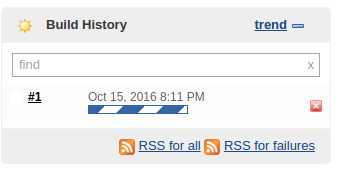
\includegraphics[scale=0.5]{build_in_progress}\\
   Si damos click sobre el build y escogemos Console Output aparecerá la consola con el progreso. La primera vez tarda bastante porque hace fetch a todo el repositorio (claramente esto es dependiente al tamaño del repositorio en cuestión). \\
   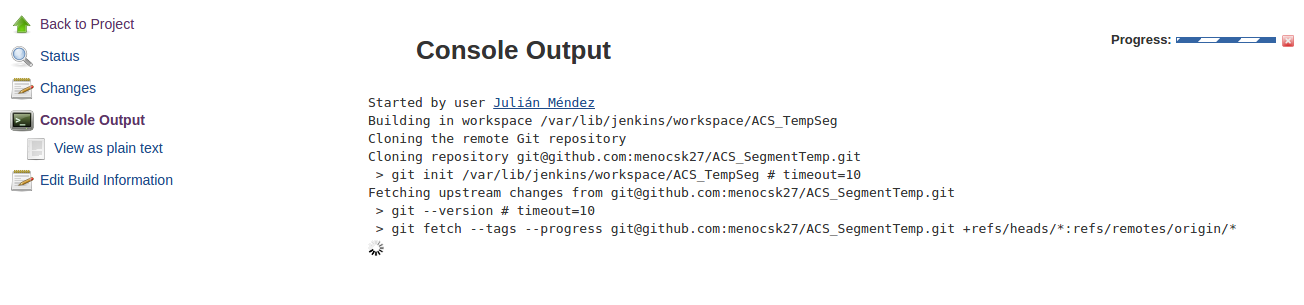
\includegraphics[scale=0.5]{progress}\\
   
   Al finalizar, veremos la gloria. \\
   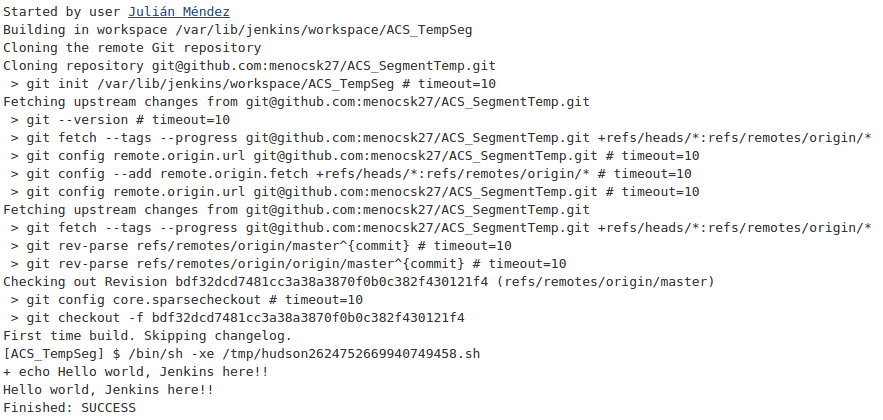
\includegraphics[scale=0.5]{glory}\\
   
   La idea es que en el comando donde de momento hay un echo puedan escribirse n pruebas unitarias que hacer con el código antes de un commit, pero de momento no tenemos pruebas unitarias de este tipo. Un ejemplo útil de algo que podemos escribir en lugar de ese echo es el comando: \\
\tab    cp * /var/www/html/ -rf\\
\tab    sudo /etc/init.d/apache2 restart\\
   Con lo que se reinicia el server de apache cada vez. \\
 
 	\textbf{Créditos:} La información principal de cómo configurar Jenkins fue obtenida de este video \url{https://www.youtube.com/watch?v=3-BgaDa5B0g} y la guía fue en colaboración de los estudiantes William Astorga y Pedro Rodríguez, que son mucho más diestros en Linux de lo que yo planeo ser algún día. 

\justify 
\newpage
\color{Blue}
\centering{ \rule{16cm}{0.1cm} } 
\justify 
\section{\textbf{Versión actual del sistema ¿Cómo obtenerla?}}}
\color{black}
\justify

\tab Para esto necesitamos iniciar la herramienta de Git, la cual es una aplicación CLI (\textit{Command Line Interface}) que también suele ser usada encapsulada tras una aplicación gráfica como lo es Github Desktop, que es la herramienta utilizada por los miembros del equipo de desarrollo de este proyecto. \\
    
    
\begin{lstlisting}[language=bash]
  cd CarpetaCopia
  git clone https://github.com/menocsk27/ACS_SegmentTemp.git
  cd ACS_SegmentTemp
\end{lstlisting}

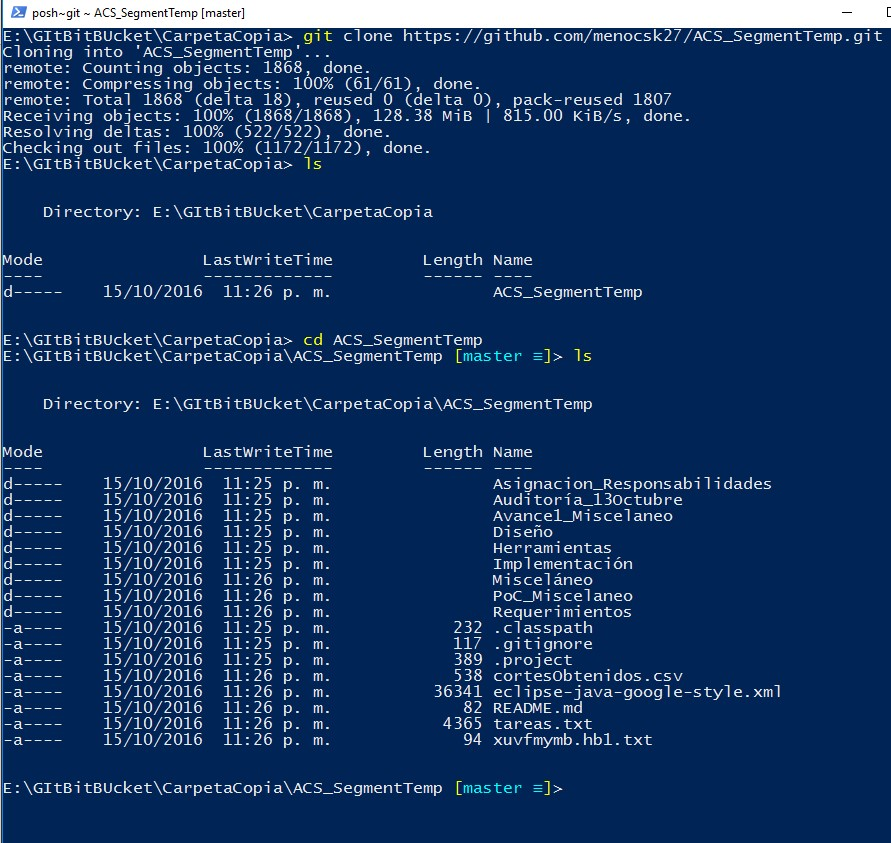
\includegraphics[scale=0.5]{git_clone.jpg}

\tab Los comandos anteriores permiten el clonado del repositorio y de su estructura general, la cual está ordenada de acuerdo al tipo de ítem de configuración de software albergados en cada carpeta. El primer comando establece la carpeta en la cual se desea alberga el repositorio, la cual llamaremos \textit{CarpetaCopia}. Para este procedimiento, \textbf{se asume que el usuario ya creó dicha carpeta}. Una vez dentro de la carpeta, procedemos a clonar el repositorio mediante el comando \textit{git clone} e insertando como parámetro la URL del repositorio. Este comando creará una carpeta con la estructura del repositorio tal y como se encuentra en la rama principal, la cual es llamada \textit{master} en Git. Este copiado o clonado del repositorio copiará todos los ítems de administración de la configuración del software a la terminal local.   \\


\justify 
\newpage
\color{Blue}
\centering{ \rule{16cm}{0.1cm} } 
\justify 
\section{\textbf{Métricas}}
\color{black}

\justify
\tab Las métricas son métodos para poder cuantificar un atributo de calidad específica de un proyecto o sistema. En el aseguramiento de la calidad del software la utilización de métricas es esencial para el mismo ya que permite mostrarle al cliente final como a demás entidades externas un valor preciso de la calidad y seguridad con la que cuenta el proyecto. En este proyecto se utilizarán distintas métricas para poder cuantificar la precisión y fiabilidad de los resultados del análisis de segmentación temporal de videos, además de qué tanta mantenibilidad se le puede dar al sistema y demás atributos de calidad externos cuantificados mediante distintas métricas, elegidas en etapas posteriores de desarrollo. \\    

Una métrica usada en este proyecto es la cuantificación de los falsos positivos y falsos negativos obtenidos tras el análisis de segmentación temporal del video y en base a un archivo ground truth subido. Esta métrica cuantifica el atributo de precisión perteneciente a la categoría de funcionalidad, según el estándar ISO-9126 de la calidad del software. La razón de el porqué se enlazó esta métrica con dicho atributo es que la función principal del video es la correcta separación del video en escenas, por lo que la precisión de los cortes debe ser elevada. Esta métrica es cuantificada en este sprint, obteniendo los valores de 2 falsos positivos (aquellos frames que sí son interpretados como cortes pero que según el archivo ground truth, no lo son) y de 372 falsos negativos. Otras de las metricas utilizadas es la complejidad ciclomática de McCabe. Esta es usada para medir el nivel de mantenibilidad del sistema, más especificamente el atributo de analizabilidad, ya que si se lleva un valor cuantificable de qué tan complejo se ha vuelto el código fuente del sistema, se podría saber qué tan factible es que ocurran errores en etapas de mantenimiento debido a lo innecesriamente complejo del mismo. El promedio de la complejidad ciclomática en el proyecto fue de 1.3. \\

La complejidad ciclomática es medida en este proyecto utilizando el plug-in \textbf{\textit{Metrics}} para Eclipse, la versión más reciente para la entrega d e este documento es la 1.3.6.\\ 

\textbf{Instalación del plug-in:}
\begin{itemize}
  \item En eclipse abrir el menú de ayuda, en este seleccionar la opción de ''Install New Software''
\end{itemize}
\centering
  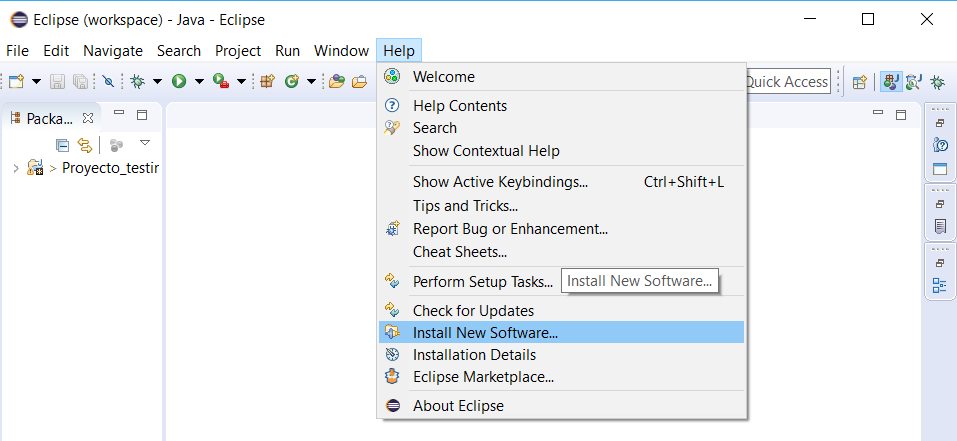
\includegraphics[scale=0.5]{Instalacion_1}
\begin{itemize}
  \item En la ventana emergente hacer click al botón de la opción ''Add...''
  \item Poner un nombre significativo, ej: Metrics 1.3.6, y en la opción de locatión poner:  $http://metrics.sourceforge.net/update$
  \item Presionar ''Ok''
\end{itemize}
  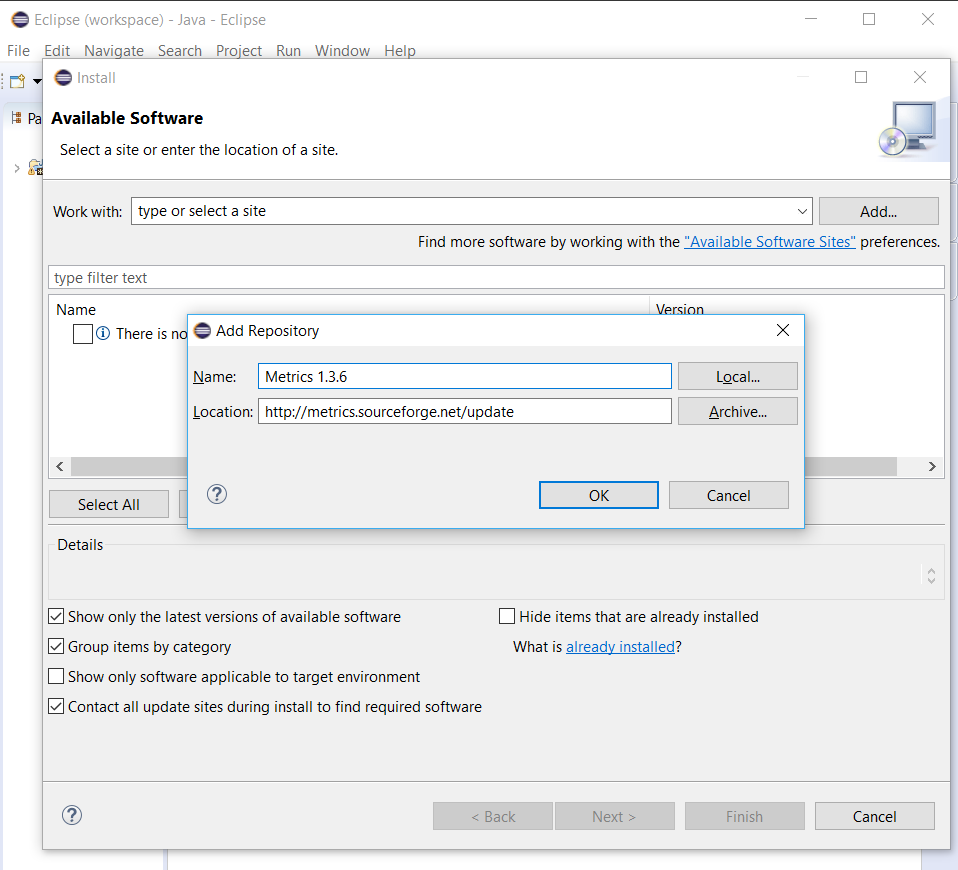
\includegraphics[scale=0.5]{Instalacion_2}
\begin{itemize}
  \item Esperar a que debajo de ''Name'' aparezca una opción con una flecha que dice ''Uncategorized''.
  \item Una vez que aparezca la opción mencionada en el punto anterior marcar el cuadro blanco para que aparezca un check. Presionar el botón ''Next''
  \item Presionar el botón de ''Next'', aceptar los terminos y condiciones
  \item Presionar el botón de ''Finish''\\
\end{itemize}

\justify
\textbf{Configurar el proyecto para permitir que el plug-in genere métricas:}
\begin{itemize}
  \item En la ventana de paquetes de Eclipse, hacer click derecho al proyecto del que se quiere generar métricas.
  \item Abrir las propiedades del proyecto y navegar al menú de ''Metrics''
  \item Marcar la opción de ''Enable Metrics''
  \item Presionar el botón de ''OK''
\end{itemize}
\centering
  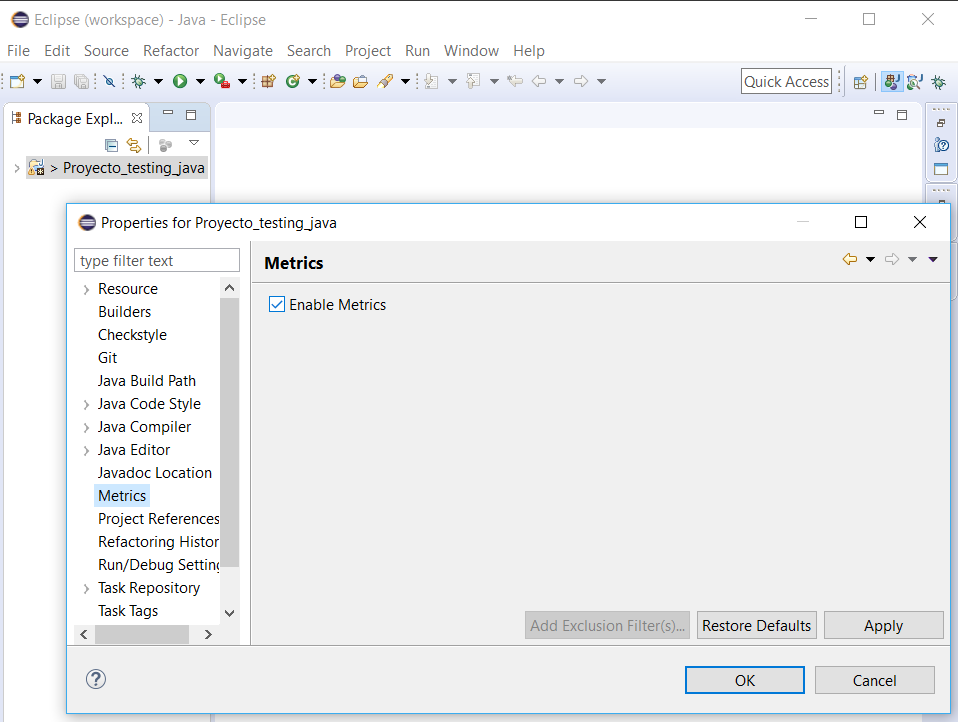
\includegraphics[scale=0.5]{Configuracion_1}

\justify
\tab De esta forma se ha configurado el proyecto de forma tal que cada vez que se compile se generen las métricas que permite Metrics 1.3.6.\\ \\ 
\textbf{Para ver las métricas generadas:}
\begin{itemize}
  \item Navegar al menú de forma: Window - Show View - Other...
  \item Buscar la carpeta de Metrics
  \item Seleccionar Metric View y presionar el botón de OK
\end{itemize} 

\begin{figure}
  \centering
  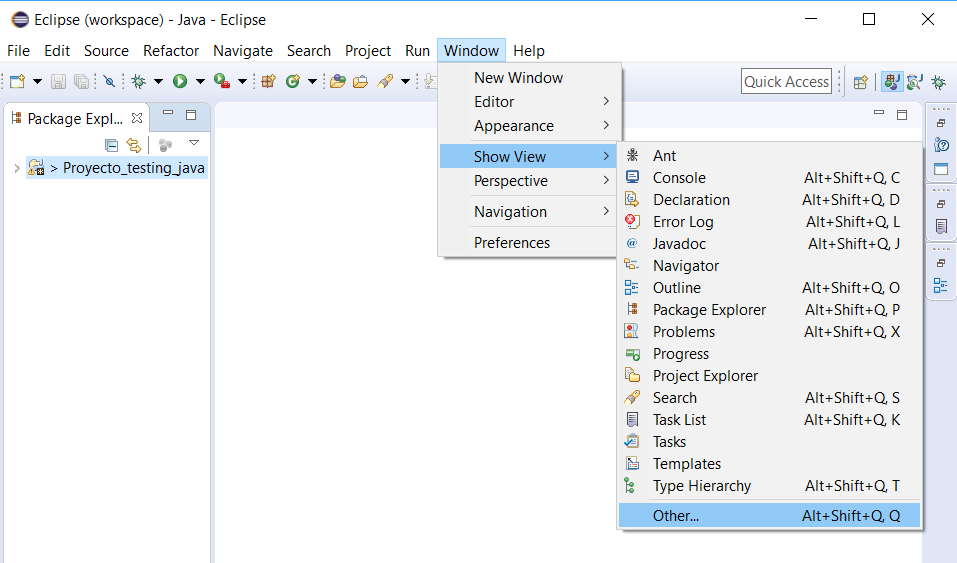
\includegraphics[scale=0.5]{Mostrar_1}
\end{figure}

\begin{figure}
  \centering
  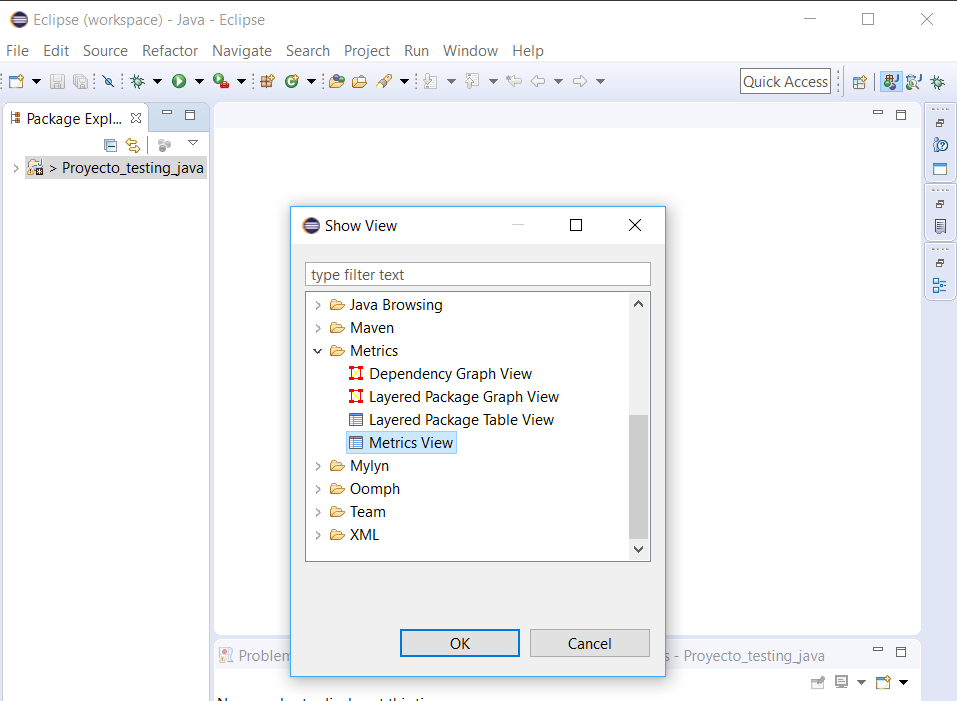
\includegraphics[scale=0.5]{Mostrar_2}
\end{figure}

\begin{figure}
  \centering
  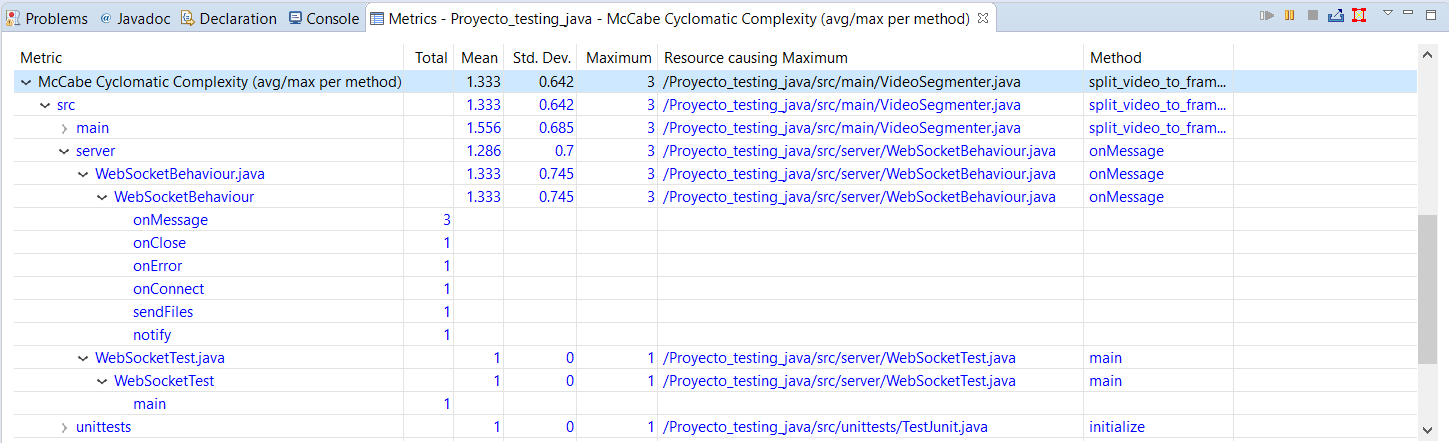
\includegraphics[scale=0.5]{Mostrar_3}
  \caption{La imagen es un ejemplo de como se ve la Complejidad Ciclomática de McCabe dado por Metrics 1.3.6.}
\end{figure}
\newpage
\color{Blue}

\centering{ \rule{16cm}{0.1cm} \\ 
\justify
\section{\textbf{Pruebas Unitarias}}
\color{black}

\justify

\tab En esta sección se definen un conjunto de pruebas unitarias realizadas para este proyecto. Dichas pruebas unitarias fueron realizadas utilizando el framework de testeo \textbf{JUnit}. Dicho framework permite la realización de pruebas unitarias y de integración de una manera simplificada y ordenada en el mismo entorno de desarrollo utilizado para la implementación general del proyecto, en este caso \textbf{Eclipse}. A continuación, se muestra la estructura general de cuatro pruebas unitarias implementadas para este avance. Se recuerda que una prueba unitaria es una prueba que valida la correcta funcionalidad de un método o función específica del código, en este caso y al implementarse el proyecto en lenguaje java, una prueba unitaria validará el correcto funcionamiento de un método. 

\begin{itemize}
\item \textbf{Prueba 1} \\  \\  
\textbf{Método a evaluar:} \textit{VideoSegmenter.splitVideosToHSV()}\\  
\textbf{Entradas esperadas: } Dirección local de un archivo de video mp4 o avi.  \\  
\textbf{Entradas atípicas: } Dirección local de un archivo no multimedia o un archivo inexistente. \\  
\textbf{Salidas: }Conjunto de objetos MAT que representan los frames hsv del video ingresado mediante ruta. \\


\item \textbf{Prueba 2} \\  \\  
\textbf{Método a evaluar:  }\textit{CsvGroundtruthreader.getAbsolutecuts()}\\  
\textbf{Entradas esperadas: }Dirección local de un archivo groundtruth csv con los rangos de los cortes en el video. \\  
\textbf{Entradas atípicas: }Dirección local de un archivo que no sea formato csv o inexistente. \\  
\textbf{Salidas: }Conjunto de Tuplas que indican el frame inicial y final de cada corte.  \\


\item \textbf{Prueba 3} \\  \\  
\textbf{Método a evaluar:} \textit{StadisticalCalculator.calculateStdDeviation()}\\  
\textbf{Entradas esperadas: Conjunto no vacío de valores decimales.} \\  
\textbf{Entradas atípicas: Conjunto vacío de valores decimales o conjunto   } \\  
\textbf{Salidas: } Valor flotante que indica la desviación estándar del conjunto ingresado como parámetro.\\ 


\item \textbf{Prueba 4} \\  \\  
\textbf{Método a evaluar:} \textit{StadisticalCalculator.calculateAverage()}\\  
\textbf{Entradas esperadas: Conjunto no vacío de valores decimales.} \\  
\textbf{Entradas atípicas: Conjunto vacío de valores decimales o conjunto   } \\  
\textbf{Salidas: } Valor flotante que indica la media del conjunto ingresado como parámetro.
\end{itemize}

	
\centering

\newpage 
% Quitar predeterminado de bibliografía article =======
\def\bibindent{1em}
\centering \color{Blue}
\begin{thebibliography}{99\kern\bibindent}
\makeatletter
\def\@biblabel#1{}
\let\old@bibitem\bibitem
\def\bibitem#1{\old@bibitem{#1}\leavevmode\kern-\bibindent}
\makeatother
\color{black}
% =====================================================

% Items =============================================== 
\bibitem{}
	\color{Blue}
	\centering \rule{13cm}{0.1cm} \\ 
    \color{Black}
    \justify
    
\bibitem{}
	Gamma, E., Helm, R., Johnson, R., \& Vlissides, J. (n.d.). \textit{Design Patterns: Elements of Reusable Object-Oriented Software} (Addison-Wesley Professional Computing Series).

\bibitem{}
	DevOps Library \textit{Using Source Control in Jenkins: DevOps Library Jenkins} \\Obtenido de: \url{https://www.youtube.com/watch?v=3-BgaDa5B0g} el 10 de octubre de 2016.
  
\end{thebibliography}

% =====================================================

\end{document}